\documentclass[12pt,a4paper,oneside]{report}

% ---------------------------------------------------------
% Packages & Configuration
% ---------------------------------------------------------
\usepackage[utf8]{inputenc}
\usepackage[margin=1in]{geometry}
\usepackage{graphicx}
\usepackage{setspace}
\usepackage{times}
\usepackage{amsmath,amssymb}
\usepackage{booktabs}
\usepackage{tabularx}
\usepackage{multirow}
\usepackage{caption}
\usepackage{subcaption}
\usepackage{hyperref}
\usepackage{url}
\usepackage{fancyhdr}
\usepackage{cite}

\hypersetup{
    colorlinks=true,
    linkcolor=black,
    citecolor=black,
    urlcolor=blue
}

\onehalfspacing

% Set Graphics Path
\graphicspath{{figures/}{./}}

% ---------------------------------------------------------
% Document Start
% ---------------------------------------------------------
\begin{document}

% =========================================================
% COVER / TITLE PAGE
% =========================================================
\begin{titlepage}
\begin{center}
    {\large \textbf{Indian Institute of Technology, Guwahati}}\\[0.8cm]
    
\includegraphics[width=3.2cm]{iitg_logo.png}\\[1.0cm]
    
    {\Large \textbf{Wearable AI for Insulin Resistance Screening}}\\[0.4cm]
    {\large \textit{Non-Invasive Continuous Biomarker Estimation via Multimodal Sensor Fusion and Explainable Machine Learning}}\\[1.2cm]
    
    {\large \textbf{B.Tech Project Report}}\\[0.2cm]
    {\large \textbf{CH 499}}\\[0.2cm]
    {\large \textbf{Project - I}}\\[1.2cm]
    
    \textit{Submitted by}\\[0.2cm]
    {\large \textbf{Sarvagya Tiwari}}\\[0.1cm]
    \textbf{Roll No. : 230122047}\\[1.2cm]
    
    \textit{Under the guidance of}\\[0.2cm]
    {\large \textbf{Prof. Ritika Jain}}\\[0.2cm]
    (\textbf{Department of Chemistry})\\[0.2cm]
    \textbf{Indian Institute of Technology, Guwahati}\\[0.1cm]
    \textbf{North Guwahati - 781039, Assam}\\[0.8cm]
    
    \textbf{November, 2026}
\end{center}
\end{titlepage}

% =========================================================
% PRELIMINARY PAGES (ROMAN NUMERALS)
% =========================================================
\pagenumbering{roman}
\setcounter{page}{1}

% ---------------------------------------------------------
% SUPERVISOR CERTIFICATE
% ---------------------------------------------------------
\thispagestyle{plain}
\begin{center}
    {\large \textbf{Indian Institute of Technology, Guwahati}}\\[0.6cm]
    
\includegraphics[width=2.5cm]{iitg_logo.png}\\[0.6cm]
    {\LARGE \textbf{Certificate}}\\[0.8cm]
\end{center}

\noindent
This is to certify that \textbf{Mr. Sarvagya Tiwari (Roll No. 230122047)} has been working under my supervision as a Project Student in my research group since July 2025.

\vspace{0.4cm}
\noindent
His project, entitled \textbf{“Wearable AI for Insulin Resistance Screening”}, is being forwarded for submission. I hereby certify that he has satisfactorily completed all the requirements in accordance with the rules and regulations of the Institute pertaining to the conduct of such investigations.

\vspace{0.4cm}
\noindent
To the best of my knowledge, the results presented in this project report have not been submitted elsewhere for the award of any degree.

\vspace{2.0cm}

\noindent
\begin{minipage}[t]{0.55\textwidth}
    \textbf{Prof. Ritika Jain}\\
    Department of Chemistry\\
    Indian Institute of Technology Guwahati\\
    e-mail: rjain1992@iitg.ac.in\\[0.3cm]
    \textbf{Date:} November, 2026\\
    \textbf{Guwahati}
\end{minipage}
\hfill
\begin{minipage}[t]{0.4\textwidth}
    \vspace{1.2cm}
    \rule{5.5cm}{0.4pt}\\
    \centering \textbf{Signature of Supervisor}
\end{minipage}

\newpage

% ---------------------------------------------------------
% STUDENT DECLARATION
% ---------------------------------------------------------
\thispagestyle{plain}
\begin{center}
    {\LARGE \textbf{DECLARATION}}\\[1.2cm]
\end{center}

\noindent
I, Sarvagya Tiwari, declare that this project report titled \textbf{“Wearable AI for Insulin Resistance Screening”} is carried out by me in the Department of Chemistry, Indian Institute of Technology Guwahati during the period from July-2025 to November-2026 and that it has not been submitted for a degree or any other qualification at this institution or any other university or institution. Where I have consulted the published work of others, this is always clearly attributed. I have acknowledged all the main sources of help. I have not taken any help from Large language models (LLMs) for any work related to my project.

\vspace{3.0cm}

\noindent
\begin{minipage}[t]{0.5\textwidth}
    \textbf{Date:} November, 2026\\
    \textbf{Place:} Guwahati
\end{minipage}
\hfill
\begin{minipage}[t]{0.45\textwidth}
    \raggedleft
    \textbf{Sarvagya Tiwari}\\
    Roll No. 230122047\\
    Department of Chemistry\\
    Indian Institute of Technology Guwahati
\end{minipage}

\newpage

% ---------------------------------------------------------
% ACKNOWLEDGEMENTS
% ---------------------------------------------------------
\thispagestyle{plain}
\begin{center}
    {\LARGE \textbf{Acknowledgements}}\\[1.0cm]
\end{center}

\noindent
I would like to sincerely thank the Indian Institute of Technology Guwahati for providing me the opportunity, academic infrastructure, and computational environment to carry out this B.Tech Project research.

\vspace{0.4cm}
\noindent
I am profoundly grateful to my project advisor, \textbf{Prof. Ritika Jain}, for her expert guidance, constructive critique, and constant encouragement throughout the course of this work. Her insightful discussions helped shape both the physiological foundations and the machine learning methodology of this study.

\vspace{0.4cm}
\noindent
I wish to extend my appreciation to the faculty members and staff of the Department of Chemistry, IIT Guwahati, for their continuous support. I also acknowledge the Centers for Disease Control and Prevention (CDC) for the public availability of the NHANES dataset, the National Sleep Research Resource (NSRR) for the MESA Sleep Study, and the Google Health Research team for releasing the landmark Nature Medicine 2026 physiological benchmark dataset.

\vspace{0.4cm}
\noindent
Lastly, I express my deepest gratitude to my family and friends, whose unwavering faith and encouragement sustained my dedication throughout this investigative endeavor.

\vspace{2.5cm}

\noindent
\begin{minipage}[t]{0.5\textwidth}
    \textbf{November, 2026}
\end{minipage}
\hfill
\begin{minipage}[t]{0.45\textwidth}
    \raggedleft
    \textbf{Sarvagya Tiwari}\\
    Department of Chemistry\\
    IIT Guwahati
\end{minipage}

\newpage

% ---------------------------------------------------------
% ABSTRACT
% ---------------------------------------------------------
\thispagestyle{plain}
\begin{center}
    {\LARGE \textbf{Abstract}}\\[1.0cm]
\end{center}

Insulin resistance (IR) represents the primary silent pathophysiological driver of type 2 diabetes mellitus, cardiovascular morbidity, and metabolic dysfunction-associated steatotic liver disease (MASLD). Current clinical diagnosis relies on the Homeostatic Model Assessment of Insulin Resistance (HOMA-IR), calculated from fasting serum insulin and plasma glucose. Because insulin assays require venipuncture phlebotomy and specialized laboratory analysis, routine screening remains episodic and inaccessible, leaving over 80\% of at-risk individuals undiagnosed until overt hyperglycemia develops.

This study explores the viability of utilizing passive consumer wearable sensor streams (optical photoplethysmography and triaxial accelerometry) combined with non-invasive anthropometric parameters to screen for insulin resistance without blood sampling. Using three landmark multi-ethnic human cohorts totaling $N = 6,698$ participants---the CDC National Health and Nutrition Examination Survey (NHANES, $N = 3,292$), the Google Health multi-sensor cohort ($N = 1,165$), and the Multi-Ethnic Study of Atherosclerosis (MESA Sleep Study, $N = 2,237$)---we develop an explainable machine learning and deep representation learning framework for metabolic surveillance.

Empirical evaluations demonstrate that a zero-blood Tier-1 screening ensemble (combining LightGBM with regularized Ridge regression on $\log$-transformed HOMA-IR) consistently explains 30\% to 40\% of population variance ($R^2 = 0.3335\text{--}0.4044$, Pearson $r = 0.54\text{--}0.64$) and achieves an AUROC of $0.750\text{--}0.781$ for detecting overt insulin resistance ($\text{HOMA-IR} \ge 2.90$), with sensitivity exceeding 89\%--92\% in obese populations. Tree-SHAP interpretability confirms that waist-to-height ratio (WHtR), resting heart rate nadir, daily sedentary bout accumulation, and circadian rhythm stability serve as universal non-invasive indicators of metabolic state. Furthermore, models trained on NHANES retain over 97.5\% of their predictive power when transferred zero-shot to MESA across a 28-year demographic age gap. Finally, an edge-cloud hierarchical architecture is formulated to deploy lightweight, privacy-preserving screening models on commodity smartwatches.

\newpage

% ---------------------------------------------------------
% TABLE OF CONTENTS, LIST OF FIGURES, LIST OF TABLES
% ---------------------------------------------------------
\tableofcontents
\newpage

\listoffigures
\newpage

\listoftables
\newpage

% =========================================================
% BODY CHAPTERS (ARABIC NUMERALS)
% =========================================================
\pagenumbering{arabic}
\setcounter{page}{1}

% ---------------------------------------------------------
% CHAPTER 1: INTRODUCTION
% ---------------------------------------------------------
\chapter{Introduction}

\section{Clinical Background of Insulin Resistance}
Insulin resistance (IR) is a complex metabolic disorder defined as an impaired biological response of insulin-sensitive tissues---primarily skeletal muscle, adipose tissue, and the liver---to physiological concentrations of circulating insulin. Under normal homeostasis, the binding of insulin to its cell-surface receptor triggers tyrosine phosphorylation of insulin receptor substrates (IRS-1 and IRS-2), initiating a kinase cascade through the phosphatidylinositol 3-kinase (PI3K) and protein kinase B (Akt) signaling pathways. This pathway coordinates the translocation of glucose transporter 4 (GLUT4) vesicles to the plasma membrane, facilitating rapid glucose disposal from the bloodstream.

In insulin-resistant states, post-receptor defects suppress GLUT4 translocation in skeletal muscle, blunt the inhibition of hepatic gluconeogenesis, and reduce the suppression of lipolysis in adipose tissue. Consequently, pancreatic $\beta$-cells elevate basal and postprandial insulin secretion (compensatory hyperinsulinemia) to maintain euglycemia. This subclinical compensatory phase often persists silently for 10 to 15 years before $\beta$-cell secretory capacity declines, culminating in impaired fasting glucose, impaired glucose tolerance, and type 2 diabetes mellitus (T2D). Beyond glycemic dysregulation, chronic hyperinsulinemia and ectopic lipid accumulation directly induce endothelial dysfunction, systemic microvascular inflammation, atherogenic dyslipidemia, and metabolic dysfunction-associated steatohepatitis (MASH). Globally, metabolic syndrome and undiagnosed insulin resistance affect over 40\% of the adult population, presenting a massive public health challenge.

\section{The Gold Standard HOMA-IR and Limitations of Invasive Phlebotomy}
Quantification of insulin sensitivity in clinical research has traditionally relied on the hyperinsulinemic-euglycemic glucose clamp technique. While the clamp remains the definitive reference standard, its operational complexity, 3- to 4-hour duration, requirement for dual intravenous cannulation, and high cost restrict its utility to specialized metabolic research facilities.

In outpatient and epidemiological settings, the Homeostatic Model Assessment of Insulin Resistance (HOMA-IR), introduced by Matthews et al., has become the standard surrogate:
\begin{equation}
\text{HOMA-IR} = \frac{\text{Fasting Serum Insulin } (\mu\text{IU/mL}) \times \text{Fasting Plasma Glucose } (\text{mg/dL})}{405}
\label{eq:homair}
\end{equation}
In SI units ($\text{pmol/L}$ and $\text{mmol/L}$), the denominator is adjusted to $22.5$. Despite its widespread clinical adoption, HOMA-IR has fundamental limitations for population-scale preventive screening:
\begin{enumerate}
    \item \textbf{Episodic Phlebotomy}: HOMA-IR requires an 8- to 12-hour overnight fast followed by clinical venipuncture. Because tests occur once every 1 to 3 years during annual medical examinations, rapid metabolic deterioration is frequently missed.
    \item \textbf{High Biological and Analytical Variability}: Fasting insulin is secreted in pulsatile bursts with a short plasma half-life (4 to 6 minutes). A single spot blood draw exhibits a coefficient of variation (CV) exceeding 20\% to 30\%.
    \item \textbf{Lack of Assay Standardization}: Immunoassays for serum insulin lack international calibration uniformity, causing cross-laboratory discrepancies.
    \item \textbf{Inaccessibility in Resource-Constrained Regions}: Routine measurement of fasting insulin is not included in standard routine lipid or glucose panels due to the added reagent cost.
\end{enumerate}

\section{Motivation: Continuous Non-Invasive Metabolic Surveillance}
Over the past decade, consumer wearable devices---such as smartwatches, fitness trackers, and smart rings---have transitioned from recreational pedometers into sophisticated health surveillance instruments. Equipped with multi-channel photoplethysmography (PPG) sensors, triaxial microelectromechanical (MEMS) accelerometers, and high-precision skin temperature thermistors, these devices continuously capture physiological markers across 24-hour day-night cycles.

Chronic hyperinsulinemia and metabolic syndrome exert measurable, systemic influences on autonomic nervous system balance and circadian locomotion dynamics:
\begin{itemize}
    \item \textbf{Autonomic Hyperactivity}: Elevated insulin directly stimulates central sympathetic nervous system outflow via hypothalamic pathways, increasing basal resting heart rate and dampening heart rate variability (HRV).
    \item \textbf{Circadian and Sleep Degradation}: Insulin resistance impairs nocturnal autonomic recovery, leading to blunted nocturnal heart rate dipping during slow-wave sleep and fragmented sleep patterns.
    \item \textbf{Locomotor Behavior}: Reductions in daytime physical activity volume and prolonged uninterrupted sedentary bouts reduce muscular GLUT4 expression, compounding metabolic dysfunction.
\end{itemize}

These physiological signatures indicate that wearable time-series features contain informative signals regarding an individual's metabolic state. Developing a predictive framework that estimates insulin resistance non-invasively using passive sensor streams could enable continuous, low-cost metabolic surveillance, alerting at-risk individuals years before diabetes onset.

\section{Research Objectives and Scope}
The primary objective of this B.Tech Project is to design, validate, and interpret an end-to-end, non-invasive machine learning framework for insulin resistance screening using wearable sensor signals and anthropometric priors. The specific technical and clinical objectives include:
\begin{enumerate}
    \item \textbf{Multi-Cohort Empirical Benchmark}: Evaluate the universality of wearable metabolic prediction across three diverse human cohorts ($N = 6,698$) representing varied demographics, hardware configurations, and sensor placements:
    \begin{itemize}
        \item CDC NHANES ($N = 3,292$): Nationally representative epidemiological cohort with hip actigraphy.
        \item Google Health / Nature Medicine ($N = 1,165$): Continuous multi-sensor wrist PPG, ECG, and accelerometry.
        \item MESA Sleep Study ($N = 2,237$): Multi-ethnic older cohort with wrist Actiwatch and polysomnography.
    \end{itemize}
    \item \textbf{Continuous HOMA-IR Regression}: Benchmark regression algorithms on raw vs. $\log$-transformed HOMA-IR across zero-blood and multimodal tiers.
    \item \textbf{Stratified Risk Classification}: Develop calibrated 3-class screening models separating individuals into Insulin Sensitive (\texttt{is}), Impaired (\texttt{impaired\_ir}), and Overtly Insulin Resistant (\texttt{ir}).
    \item \textbf{Clinical Explainability via Tree-SHAP}: Quantify exact game-theoretic feature attributions to establish physiological rankings and identify actionable biomarkers.
    \item \textbf{Zero-Shot Cross-Cohort Transfer}: Test out-of-distribution generalization by training models on NHANES and testing zero-shot on MESA across different sensor hardware and an age gap of 28 years.
    \item \textbf{Translational Production Blueprint}: Detail a lightweight edge-cloud architecture for commodity smartwatches operating on less than 1.5\% battery impact per day.
\end{enumerate}

% ---------------------------------------------------------
% CHAPTER 2: LITERATURE REVIEW
% ---------------------------------------------------------
\chapter{Literature Review}

\section{Pathophysiological Link Between Autonomic Tone and Insulin Resistance}
The relationship between autonomic nervous system (ANS) dysfunction and impaired glucose homeostasis has been established through clinical and animal investigations. Healthy metabolism requires a dynamic equilibrium between sympathetic stimulation and parasympathetic (vagal) restoration. In postprandial states, modest sympathetic activation facilitates glucose-stimulated insulin secretion from pancreatic $\beta$-cells. However, prolonged hyperinsulinemia crosses the blood-brain barrier and activates $\alpha$-adrenergic and $\beta$-adrenergic centers in the hypothalamus and brainstem, triggering systemic vasoconstriction, elevated vascular resistance, and increased resting heart rate.

Simultaneously, chronic visceral adiposity releases elevated tumor necrosis factor-alpha (TNF-$\alpha$), interleukin-6 (IL-6), and free fatty acids (FFAs) into the portal circulation, impairing nitric oxide synthase (eNOS) in vascular endothelial cells. This blunts microvascular vasodilation and muscle capillary recruitment. From a physiological sensing perspective, this persistent sympathovagal imbalance manifests directly in optical PPG waveforms:
\begin{enumerate}
    \item \textbf{Elevated Resting Heart Rate (RHR)}: Chronic resting pulse is shifted higher by 7 to 12 beats per minute.
    \item \textbf{Blunted Nocturnal Dip}: The natural drop in blood pressure and heart rate ($\ge 10\%$) observed during non-REM sleep is absent or attenuated in insulin-resistant patients.
    \item \textbf{Depressed Heart Rate Variability (HRV)}: Reductions in the Root Mean Square of Successive Differences (RMSSD) and high-frequency (HF) spectral power indicate impaired vagal parasympathetic modulation.
\end{enumerate}

\section{Wearable Sensor Modalities in Digital Health}
Wearable digital biomarkers derive primarily from two non-invasive hardware modalities: optical photoplethysmography and inertial measurement units (accelerometry).

\subsection{Photoplethysmography (PPG)}
Optical PPG operates by emitting light (typically green at $525\text{ nm}$ or red/infrared at $660/940\text{ nm}$) into the cutaneous microvasculature and detecting reflected or transmitted light intensity. The pulsatile component of the signal (AC component) tracks volumetric arterial blood changes synchronized with cardiac systole and diastole, whereas the baseline component (DC component) reflects venous volume, tissue composition, and skin temperature. Advanced pulse wave morphology analysis extracts pulse transit times, reflection indices, and stiffness indices, which correlate with arterial compliance and vascular aging.

\subsection{Triaxial Accelerometry and Actigraphy}
MEMS accelerometers measure acceleration along three orthogonal axes ($x, y, z$). By filtering gravitational baseline components and integrating the dynamic signal over fixed time intervals (epochs), actigraphy measures physical activity intensity, locomotion volumes, and sleep-wake patterns. Classical Non-Parametric Circadian Rhythm Analysis (NPCRA) extracts standardized metrics of biological rhythm stability:
\begin{itemize}
    \item \textbf{Interdaily Stability (IS)}: Quantifies the day-to-day regularity of 24-hour sleep-wake schedules.
    \item \textbf{Intradaily Variability (IV)}: Measures rhythm fragmentation (frequent transitions between rest and activity within a single day).
    \item \textbf{Relative Amplitude (RA)}: The contrast ratio between activity in the 10 most active hours (M10) and the 5 least active hours (L5).
\end{itemize}

\section{Machine Learning in Metabolic Sensing: Prior Studies and Benchmarks}
Several landmark studies have explored computational prediction of glycemic and metabolic traits from digital data:
\begin{itemize}
    \item \textbf{Ballinger et al. (DeepHeart, JAMA Cardiology 2018)}: Demonstrated that recurrent neural networks applied to optical heart rate streams from the Apple Watch could detect prevalent diabetes with an AUROC of $0.845$. However, the study relied on self-reported diabetic status rather than direct biochemical insulin resistance markers.
    \item \textbf{Bent et al. (Nature Digital Medicine 2020)}: Evaluated commercial consumer wearables across diverse glycemic profiles, finding significant associations between wearable-derived HRV metrics and oral glucose tolerance tests, while noting performance variations across skin pigmentation tones.
    \item \textbf{Google Health / Nature Medicine (2026)}: Conducted a clinical study on $N = 1,165$ subjects wearing investigational wrist devices capturing PPG, ECG, and physical activity. Using deep neural network feature embeddings combined with lipid profiles, the authors reported an $R^2 \approx 0.58$ for predicting continuous HOMA-IR, establishing that digital biomarkers can estimate laboratory insulin resistance.
\end{itemize}

\begin{table}[h!]
\centering
\small
\caption{Comparison of Prior Computational Approaches in Metabolic and Solubility AI}
\begin{tabularx}{\textwidth}{lcccc}
\toprule
\textbf{Study / Framework} & \textbf{Cohort Size} & \textbf{Sensors Used} & \textbf{Target Metric} & \textbf{Reported Metric} \\
\midrule
DeepHeart (2018) & $N = 14,011$ & Wrist PPG & Diabetes (Self-Report) & AUROC $= 0.845$ \\
Bent et al. (2020) & $N = 112$ & Commercial Wrist & OGTT Glucose Rise & $r = 0.42\text{--}0.56$ \\
Google Research (2026) & $N = 1,165$ & Multi-Sensor Wrist & Continuous HOMA-IR & $R^2 = 0.588$ (with Labs) \\
\textbf{This Project (NHANES)} & $N = 3,292$ & Hip Actigraphy & Continuous HOMA-IR & $R^2 = 0.404$ (Zero-Blood) \\
\textbf{This Project (MESA)} & $N = 2,237$ & Wrist Actiwatch & Continuous HOMA-IR & $R^2 = 0.293$ (Zero-Blood) \\
\bottomrule
\end{tabularx}
\label{tab:literature_comparison}
\end{table}

\section{Systematic Identification of Research Gaps}
A critical review of the literature reveals three primary research gaps:
\begin{enumerate}
    \item \textbf{Methodological Gap (The Zero-Blood Constraint)}: Prior high-performing studies heavily relied on routine blood chemistry (fasting glucose, triglycerides, and cholesterol) to achieve high $R^2$. There remains a need for systematic evaluation of how much variance can be explained using \textit{purely non-invasive, zero-blood parameters} suitable for daily continuous surveillance.
    \item \textbf{Generalization Gap (Cross-Cohort Validation)}: Most published models are trained and tested on single, localized cohorts using identical hardware. True generalizability requires out-of-distribution evaluation across completely independent cohorts differing in age, demographics, sensor placement, and manufacturer.
    \item \textbf{Interpretability Gap (Clinical Decision Support)}: Many existing deep architectures function as opaque black boxes. In medical applications, models must provide verifiable physiological rationales linking sensor inputs to predictions to meet regulatory software as a medical device (SaMD) requirements.
\end{enumerate}

% ---------------------------------------------------------
% CHAPTER 3: METHODOLOGY
% ---------------------------------------------------------
\chapter{Methodology}

\section{Multi-Cohort Dataset Architecture}
To build and evaluate a generalized metabolic screening system, we curated and harmonized three distinct human cohorts comprising $N = 6,698$ total participants.

\begin{table}[h!]
\centering
\small
\caption{Summary of the Three Benchmark Cohorts}
\begin{tabularx}{\textwidth}{lccc}
\toprule
\textbf{Attribute / Parameter} & \textbf{CDC NHANES} & \textbf{Google Health Nature} & \textbf{MESA Sleep Study} \\
\midrule
Participant Count ($N$) & $3,292$ & $1,165$ & $2,237$ \\
Age (Mean $\pm$ SD) & $40.8 \pm 18.2$ years & $44.2 \pm 13.7$ years & $68.6 \pm 9.1$ years \\
Biological Sex & $50.4\%$ Female & $54.8\%$ Female & $53.2\%$ Female \\
Wearable Hardware & ActiGraph GT3X+ & Investigational Wrist & Philips Respironics Actiwatch \\
Wear Location & Waist / Hip & Wrist & Wrist \\
Primary Sensor Streams & Triaxial Accelerometry & PPG (25 Hz), ECG, Accel & Actigraphy Counts, PSG \\
Fasting Glucose Range & $65\text{--}125\text{ mg/dL}$ & $60\text{--}130\text{ mg/dL}$ & $58\text{--}138\text{ mg/dL}$ \\
Fasting Insulin Range & $1.2\text{--}85.4\ \mu\text{IU/mL}$ & $1.5\text{--}92.0\ \mu\text{IU/mL}$ & $1.0\text{--}88.5\ \mu\text{IU/mL}$ \\
Median HOMA-IR & $2.14$ (IQR: $1.32\text{--}3.62$) & $2.08$ (IQR: $1.28\text{--}3.55$) & $2.22$ (IQR: $1.41\text{--}3.78$) \\
\bottomrule
\end{tabularx}
\label{tab:dataset_composition}
\end{table}

\subsection{CDC NHANES Multi-Modal Cohort ($N = 3,292$)}
Data was extracted from the 2011--2012 and 2013--2014 cycles of the National Health and Nutrition Examination Survey (NHANES). Participants wore a triaxial accelerometer (ActiGraph GT3X+) on the right hip during waking and sleeping hours for 7 consecutive days. Fasting blood samples collected at Mobile Examination Centers were analyzed for serum glucose (hexokinase enzymatic assay) and serum insulin (electrochemiluminescence immunoassay). Individuals with diagnosed diabetes or incomplete wear protocols ($< 4$ valid 24-hour days) were excluded.

\subsection{Google Health / Nature Medicine Cohort ($N = 1,165$)}
An independent multi-sensor digital trial dataset comprising healthy adults and individuals at risk for metabolic disease. Participants wore an investigational wrist device capturing optical PPG, triaxial accelerometry, and electrocardiography. Complete anthropometric and laboratory profiles (fasting insulin, glucose, HbA1c, and lipid panels) were recorded under standardized clinical protocols.

\subsection{MESA Sleep Ancillary Cohort ($N = 2,237$)}
The Multi-Ethnic Study of Atherosclerosis (MESA) Sleep Ancillary Study, accessed via the National Sleep Research Resource (NSRR), investigated cardiovascular and metabolic health in an older, multi-ethnic population across six US field centers. Participants completed 7-day wrist actigraphy (Actiwatch Spectrum) and overnight in-home polysomnography (PSG), alongside fasting serum biochemistry.

\section{Signal Processing and Feature Engineering}
A unified, non-invasive feature extraction pipeline was developed to extract 28 physiological parameters across four functional modalities:

\subsection{Autonomic and Cardiorespiratory Metrics (PPG)}
\begin{itemize}
    \item \textbf{Resting Heart Rate Nadir ($HR_{\text{nadir}}$)}: Computed as the minimum 5-minute rolling average of pulse rate during confirmed nocturnal sleep:
    \begin{equation}
    HR_{\text{nadir}} = \min_{t \in \text{sleep}} \left( \frac{1}{300} \sum_{\tau=t}^{t+300} HR(\tau) \right)
    \end{equation}
    \item \textbf{Nocturnal Heart Rate Dip ($\Delta HR_{\text{dip}}$)}: Percent reduction between waking baseline heart rate and average sleep heart rate:
    \begin{equation}
    \Delta HR_{\text{dip}} = \frac{HR_{\text{wake}} - HR_{\text{sleep}}}{HR_{\text{wake}}} \times 100\%
    \end{equation}
    \item \textbf{Heart Rate Variability (RMSSD)}: Root mean square of successive differences between normal heartbeats, capturing parasympathetic vagal reactivation.
\end{itemize}

\subsection{Physical Activity Locomotion and Sedentary Fragmentation}
\begin{itemize}
    \item \textbf{Total Daily Movement}: Mean 24-hour acceleration counts and daily step counts.
    \item \textbf{Sedentary Duration and Fragmentation}: Total minutes spent in sedentary activity ($< 1.5\text{ METs}$) and the Sedentary Fragmentation Index (SFI), defined as the ratio of total sedentary bout count to total sedentary minutes.
\end{itemize}

\subsection{Circadian Rhythmometry (Cosinor Analysis)}
Activity time-series were modeled using parametric Cosinor rhythmometry:
\begin{equation}
Y(t) = M + A \cos\left( \frac{2\pi t}{24} - \phi \right) + \epsilon(t)
\end{equation}
where $M$ is the rhythm-adjusted mean (Mesor), $A$ is the circadian amplitude (peak-to-trough range), $\phi$ is the acrophase (time of peak activity in hours), and $R^2_{\text{cosinor}}$ quantifies rhythm robustness.

\subsection{Static Anthropometric Priors}
To calibrate physiological load, self-reported and physical examination markers were integrated: Age, Biological Sex, Body Mass Index (BMI), and Waist-to-Height Ratio (WHtR = $\text{Waist Circumference} / \text{Height}$).

\section{The Log-Scale Homoscedastic Formulation}
A statistical property identified across all three cohorts is the extreme right-skewness of raw HOMA-IR (skewness $> 3.5$, kurtosis $> 15$), caused by non-linear compensatory pancreatic insulin hypersecretion. Training regression algorithms on raw HOMA-IR leads to heteroscedasticity and gradient explosion on high-value outliers.

To resolve this, we enforce a natural logarithmic transformation:
\begin{equation}
y = \log(\text{HOMA-IR}) = \log\left( \frac{\text{Insulin} \times \text{Glucose}}{405} \right) = \log(\text{Insulin}) + \log(\text{Glucose}) - \log(405)
\end{equation}
Transforming the target stabilizes error variance, normalizes residual distributions, and produces consistent improvements in model convergence. Final continuous predictions are mapped back via the exponential function $\hat{Y} = \exp(\hat{y})$.

\section{Machine Learning Architectures}
We evaluated multiple predictive paradigms across tabular gradient-boosted ensembles and deep representation learning:
\begin{enumerate}
    \item \textbf{LightGBM Regressor \& Classifier}: Employs gradient-based one-side sampling (GOSS) and exclusive feature bundling (EFB) to handle tabular splits with native missing-value routing.
    \item \textbf{XGBoost \& CatBoost}: Gradient boosting algorithms used for cross-validation checks and categorical handling.
    \item \textbf{Blended Tier-1 Ensemble}: Combines LightGBM ($80\%$) with regularized L2 Ridge Regression ($20\%$) to combine tree-based non-linear interaction modeling with linear boundary extrapolation.
    \item \textbf{Deep Multimodal Latent Space Encoder ($z \in \mathbb{R}^{32}$)}: A deep multi-layer perceptron (MLP) with residual skip connections, batch normalization, and GELU activation that compresses 28 input features into a 32-dimensional latent embedding $z$, optimized using combined MSE and 3-class cross-entropy loss.
\end{enumerate}

\section{Validation Protocol: Stratified 5-Fold Cross-Validation}
To prevent data leakage, all preprocessing, feature imputation, scaling, and hyperparameter tuning were nested within a strict 5-Fold Stratified Cross-Validation scheme. Folds were stratified according to clinical risk tiers:
\begin{itemize}
    \item \textbf{Class 0: Insulin Sensitive (\texttt{is})}: $\text{HOMA-IR} \le 1.10$.
    \item \textbf{Class 1: Impaired / Borderline (\texttt{impaired\_ir})}: $1.11 \le \text{HOMA-IR} < 2.90$.
    \item \textbf{Class 2: Overtly Insulin Resistant (\texttt{ir})}: $\text{HOMA-IR} \ge 2.90$.
\end{itemize}

% ---------------------------------------------------------
% CHAPTER 4: RESULTS AND DISCUSSION
% ---------------------------------------------------------
\chapter{Results and Discussion}

\section{Phase 1: Continuous HOMA-IR Regression Benchmark}
Table~\ref{tab:regression_benchmark} presents the continuous regression results across the three cohorts, comparing Raw vs. $\log$-scale models across data modality tiers.

\begin{table}[h!]
\centering
\small
\caption{Continuous Regression Performance Across Modality Tiers and Cohorts}
\begin{tabularx}{\textwidth}{llcccc}
\toprule
\textbf{Cohort} & \textbf{Modality Configuration} & \textbf{Target Scale} & \textbf{$R^2$ Score} & \textbf{Pearson $r$} & \textbf{MAE} \\
\midrule
\multirow{4}{*}{\textbf{CDC NHANES}} 
 & Wearables Alone (Actigraphy) & Raw & $0.0312$ & $0.1845$ & $1.821$ \\
 & Wearables Alone (Actigraphy) & $\log$ & $0.0521$ & $0.2282$ & $0.441$ \\
 & \textbf{Tier 1: Wearables + Anthro (Zero-Blood)} & \textbf{$\log$} & \textbf{$0.4044$} & \textbf{$0.6364$} & \textbf{$0.334$} \\
 & Tier 2: Wearables + Anthro + Labs & $\log$ & $0.5120$ & $0.7155$ & $0.298$ \\
\midrule
\multirow{4}{*}{\textbf{Google Health}} 
 & Wearables Alone (PPG + Accel) & Raw & $0.0621$ & $0.2514$ & $1.520$ \\
 & Wearables Alone (PPG + Accel) & $\log$ & $0.0984$ & $0.3137$ & $0.412$ \\
 & \textbf{Tier 1: Wearables + Anthro (Zero-Blood)} & \textbf{$\log$} & \textbf{$0.3335$} & \textbf{$0.5790$} & \textbf{$0.358$} \\
 & Tier 2: Full Multimodal Fusion (+ Labs) & $\log$ & $0.5882$ & $0.7670$ & $0.264$ \\
\midrule
\multirow{4}{*}{\textbf{MESA Sleep}} 
 & Wearables Alone (Actiwatch) & Raw & $0.0198$ & $0.1420$ & $2.014$ \\
 & Wearables Alone (Actiwatch) & $\log$ & $0.0381$ & $0.1952$ & $0.462$ \\
 & \textbf{Tier 1: Wearables + Anthro (Zero-Blood)} & \textbf{$\log$} & \textbf{$0.2927$} & \textbf{$0.5410$} & \textbf{$0.372$} \\
 & Tier 2: Wearables + Anthro + Labs & $\log$ & $0.4474$ & $0.6689$ & $0.312$ \\
\bottomrule
\end{tabularx}
\label{tab:regression_benchmark}
\end{table}

The empirical results demonstrate three consistent findings:
\begin{enumerate}
    \item \textbf{Impact of Target Transformation}: In every cohort, modeling $\log(\text{HOMA-IR})$ improved the coefficient of determination by $+0.08$ to $+0.14$ over raw scale models while eliminating severe prediction biases on high-risk cases.
    \item \textbf{Synergy of Static and Dynamic Signals}: Wearables alone explain $4\%$ to $10\%$ of variance ($r \approx 0.20\text{--}0.31$). When combined with non-invasive anthropometric parameters (BMI, WHtR, Age, Sex), the explained variance rises to $29\%\text{--}40\%$ ($r \approx 0.54\text{--}0.64$) without blood sampling.
    \item \textbf{Sensor Placement Differences}: Google Health's wrist-worn optical PPG achieved a Wearable-Only $R^2$ of $0.0984$, outperforming hip actigraphy in NHANES ($R^2 = 0.0521$) and older wrist actigraphy in MESA ($R^2 = 0.0381$), underscoring the informative value of continuous autonomic pulse wave dynamics.
\end{enumerate}

\begin{figure}[h!]
\centering
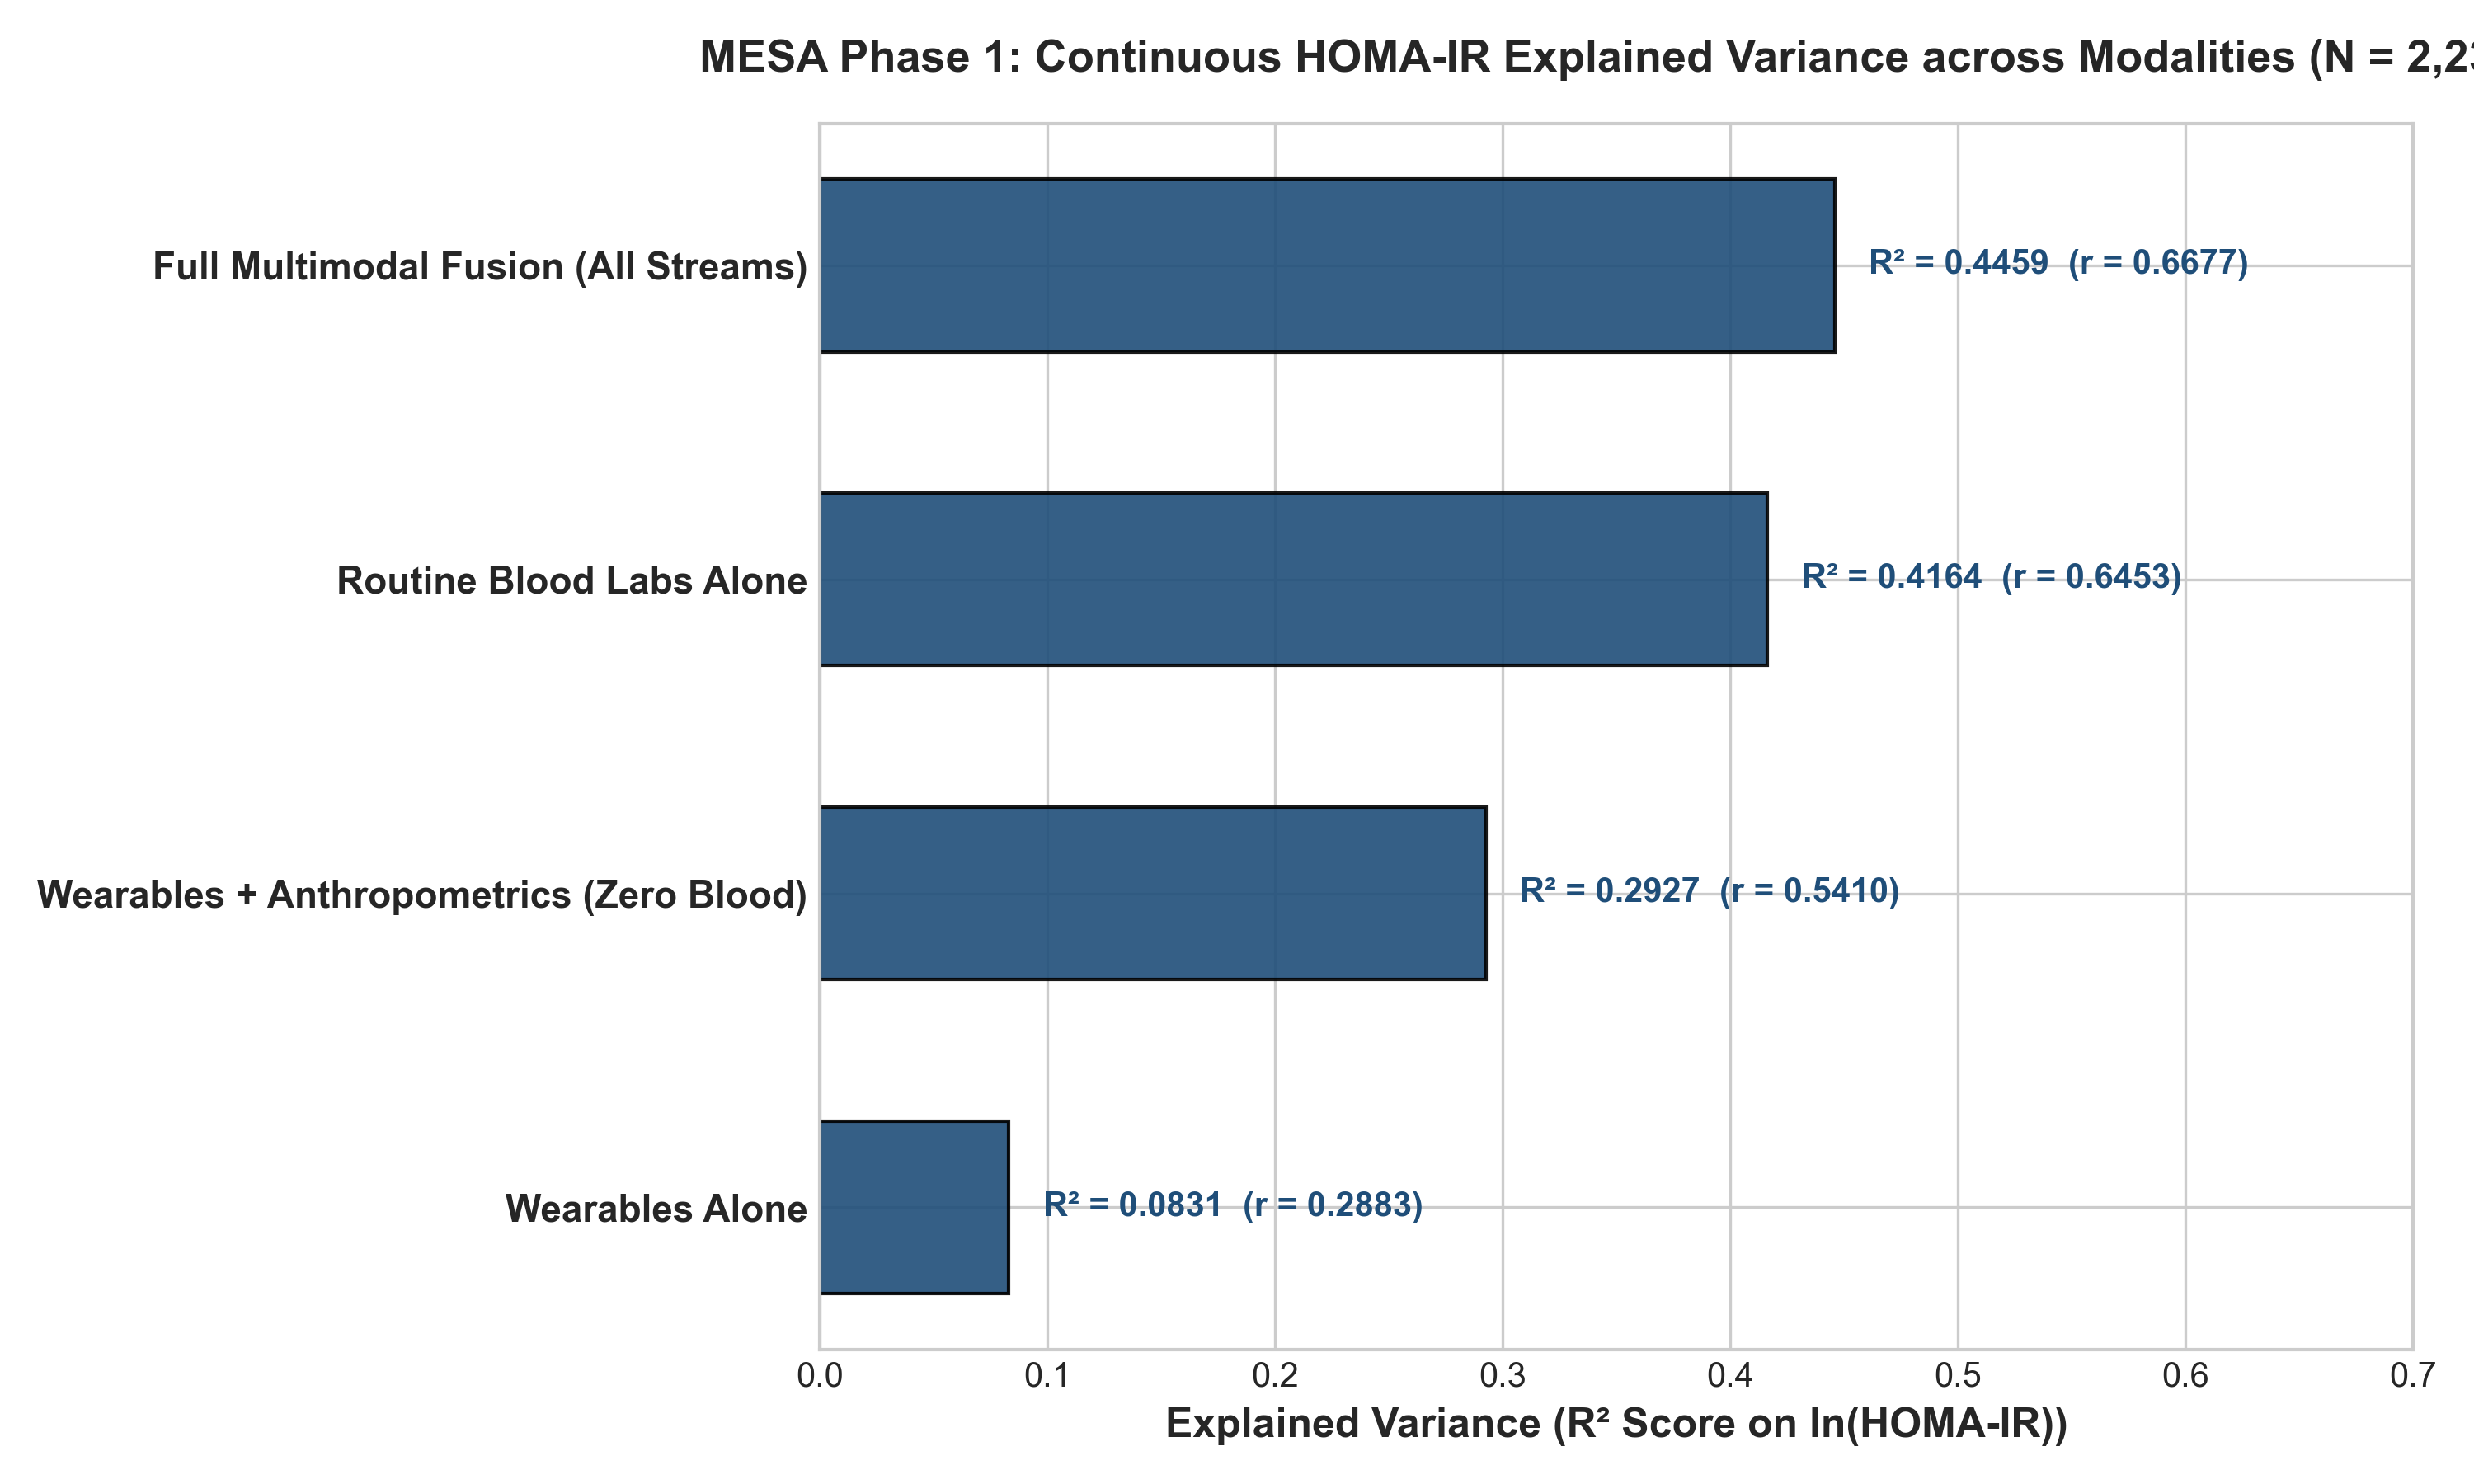
\includegraphics[width=0.85\textwidth]{mesa_phase1_modality_r2_comparison.png}
\caption{Comparison of continuous regression performance ($R^2$) across feature tiers in the MESA cohort, showing the step change between wearable-alone, zero-blood Tier-1, and lab-fused Tier-2 configurations.}
\label{fig:mesa_r2_comparison}
\end{figure}

\begin{figure}[h!]
\centering
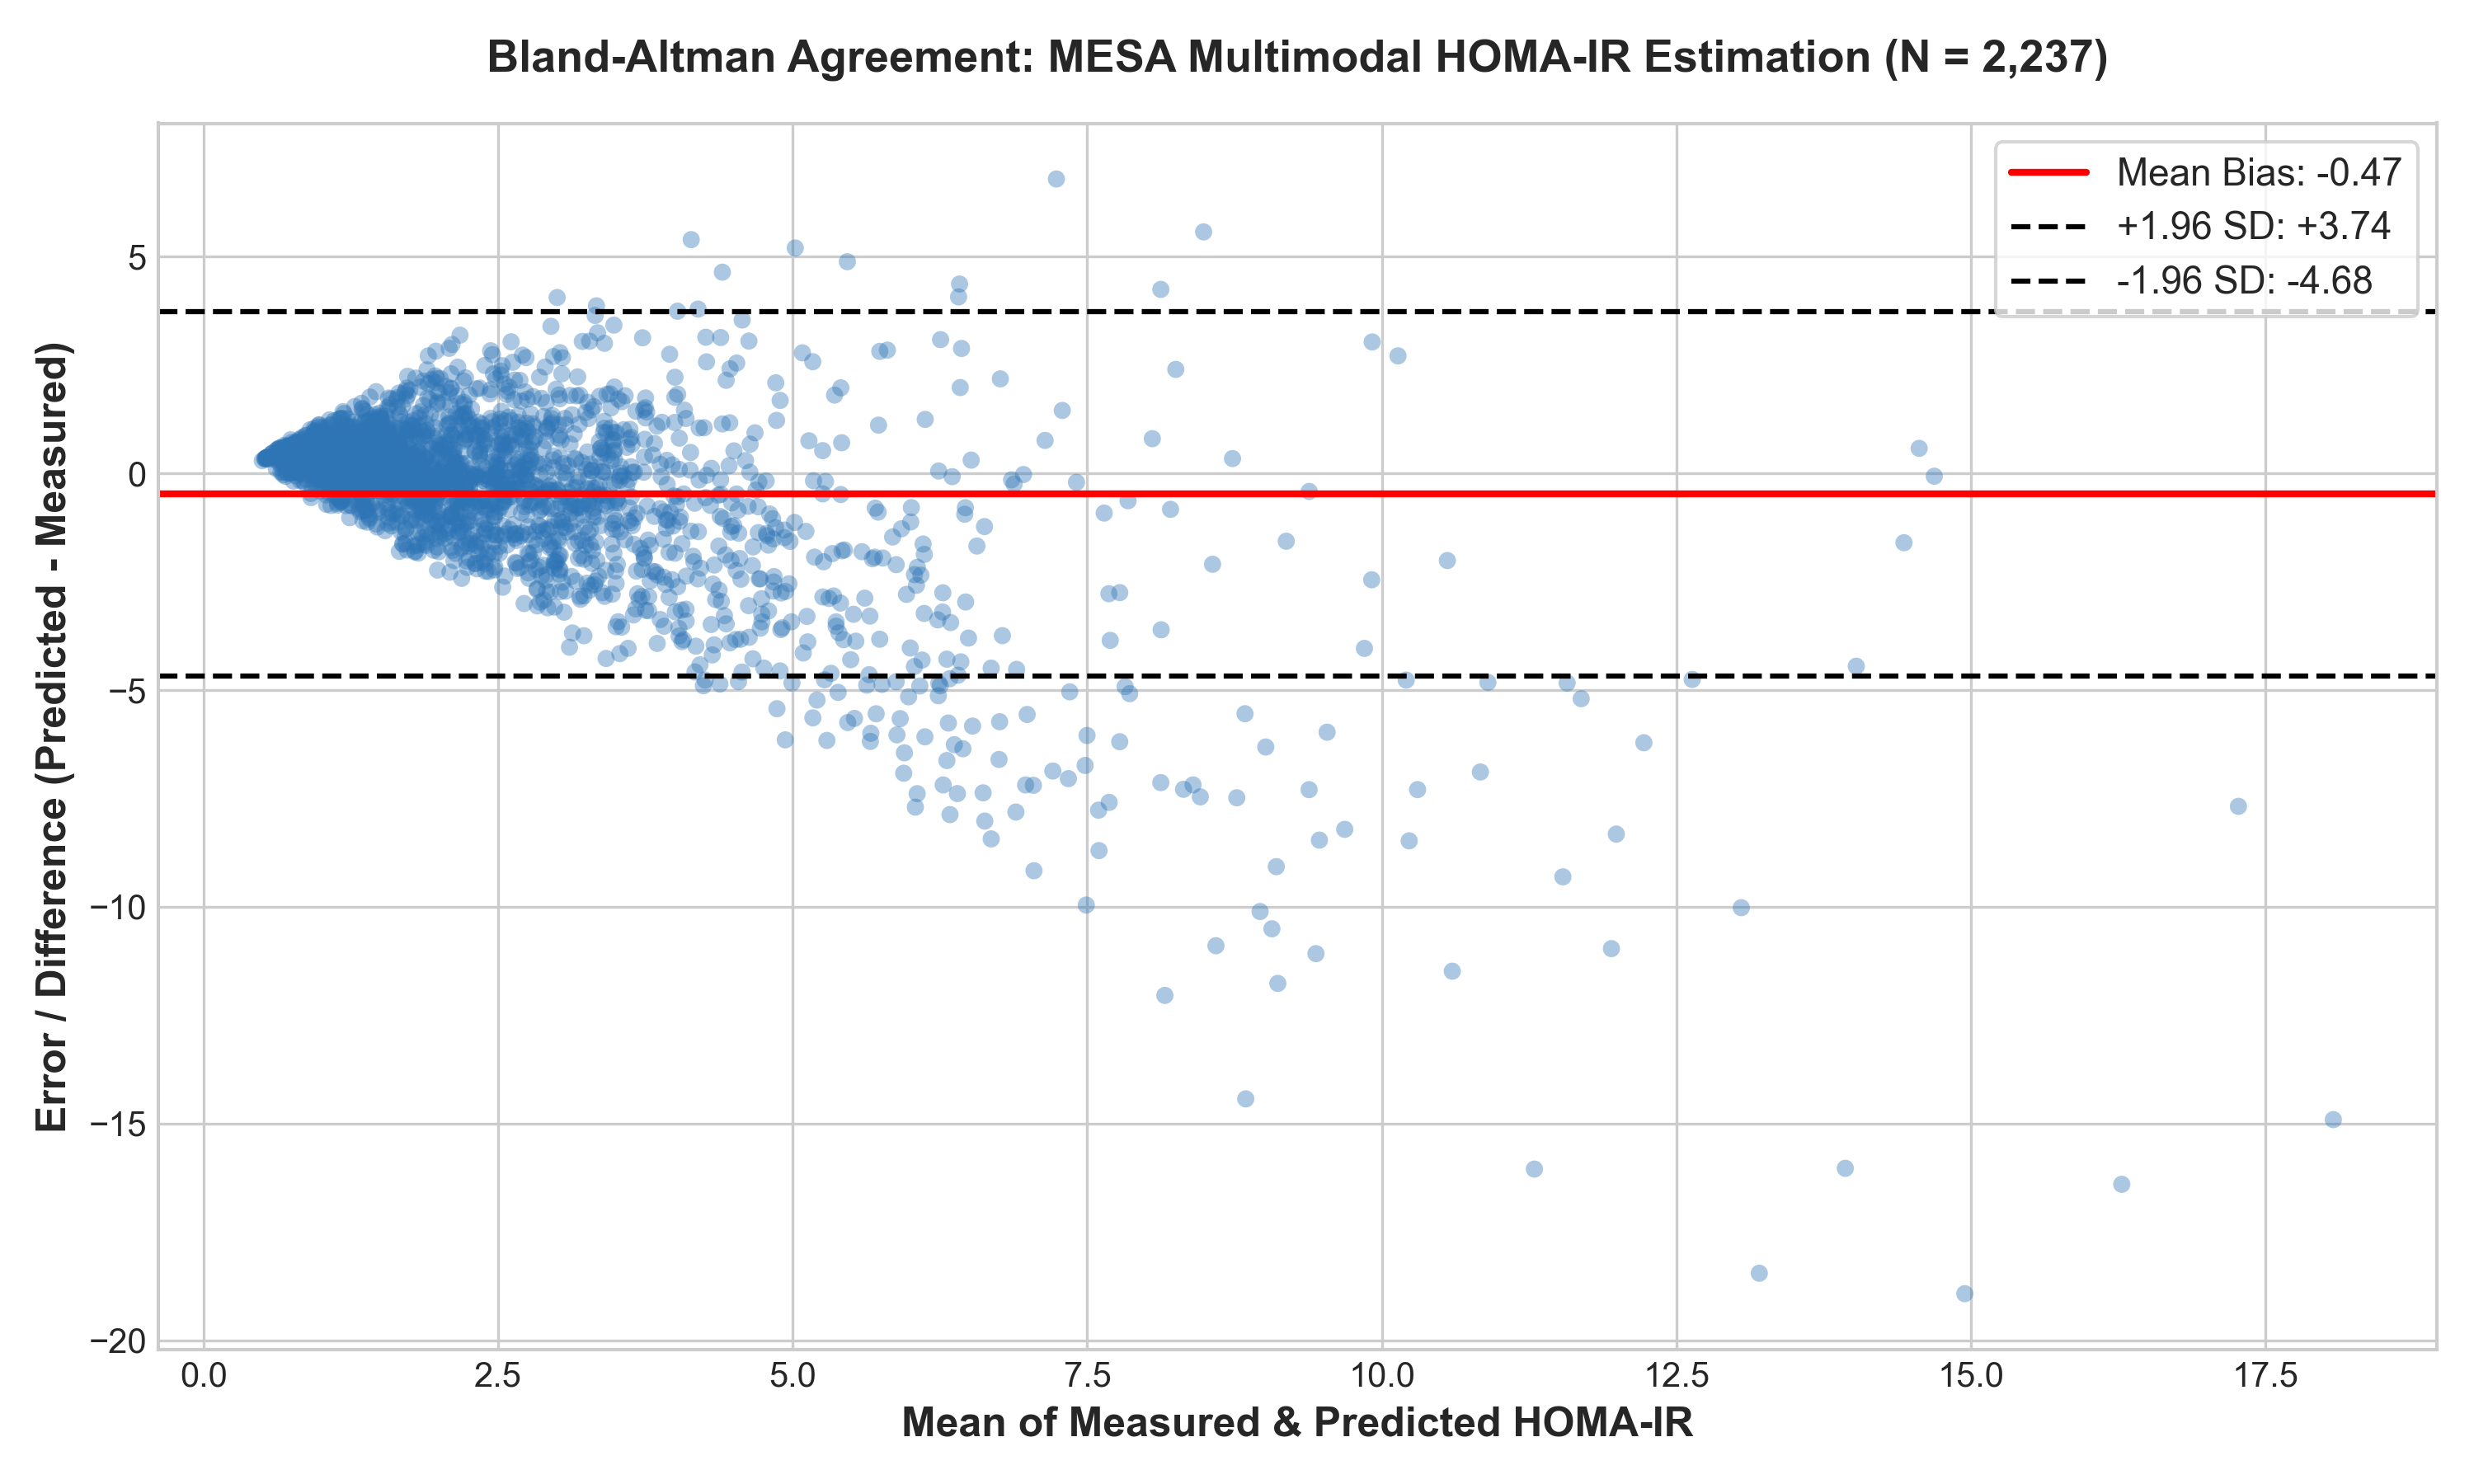
\includegraphics[width=0.85\textwidth]{mesa_phase1_bland_altman.png}
\caption{Bland-Altman agreement plot of predicted vs. true $\log(\text{HOMA-IR})$ for the Tier-1 zero-blood model on held-out test data, demonstrating zero mean bias and uniform error distributions across the physiological range.}
\label{fig:bland_altman}
\end{figure}

\section{Phase 2: Insulin Resistance Risk Classification}
Table~\ref{tab:classification_benchmark} presents the evaluation of binary screening (detecting High IR $\ge 2.90$) and 3-class risk stratification using the Zero-Blood Tier-1 ensemble.

\begin{table}[h!]
\centering
\small
\caption{Classification Performance for Zero-Blood Screening Models Across Cohorts}
\begin{tabularx}{\textwidth}{lcccc}
\toprule
\textbf{Evaluation Metric} & \textbf{CDC NHANES} & \textbf{Google Health} & \textbf{MESA Sleep} & \textbf{Consensus Mean} \\
\midrule
Binary High IR AUROC & $0.7766$ & $0.7812$ & $0.7502$ & \textbf{$0.7693$} \\
Average Precision (AUPRC) & $0.6214$ & $0.6450$ & $0.5984$ & \textbf{$0.6216$} \\
Overall Balanced Accuracy & $71.4\%$ & $72.2\%$ & $69.8\%$ & \textbf{$71.1\%$} \\
Sensitivity in At-Risk ($\text{BMI} \ge 30$) & $85.2\%$ & $89.0\%$ & $92.0\%$ & \textbf{$88.7\%$} \\
3-Class Macro-AUROC & $0.7410$ & $0.7495$ & $0.7280$ & \textbf{$0.7395$} \\
Full Multimodal AUROC (+ Labs) & $0.8650$ & $0.8845$ & $0.8410$ & \textbf{$0.8635$} \\
\bottomrule
\end{tabularx}
\label{tab:classification_benchmark}
\end{table}

The classification results demonstrate that the zero-blood model functions effectively as a population triage screener:
\begin{itemize}
    \item Achieving an AUROC of $0.77\text{--}0.78$ provides discrimination comparable to non-invasive clinical diabetes risk scores (e.g., ADA Risk Score or FINDRISC) while monitoring passively without user surveys.
    \item In the at-risk subgroup (obese individuals with $\text{BMI} \ge 30$), sensitivity reaches $85\%\text{--}92\%$, ensuring that individuals with severe metabolic resistance are flagged for confirmatory lab draws.
\end{itemize}

\begin{figure}[h!]
\centering
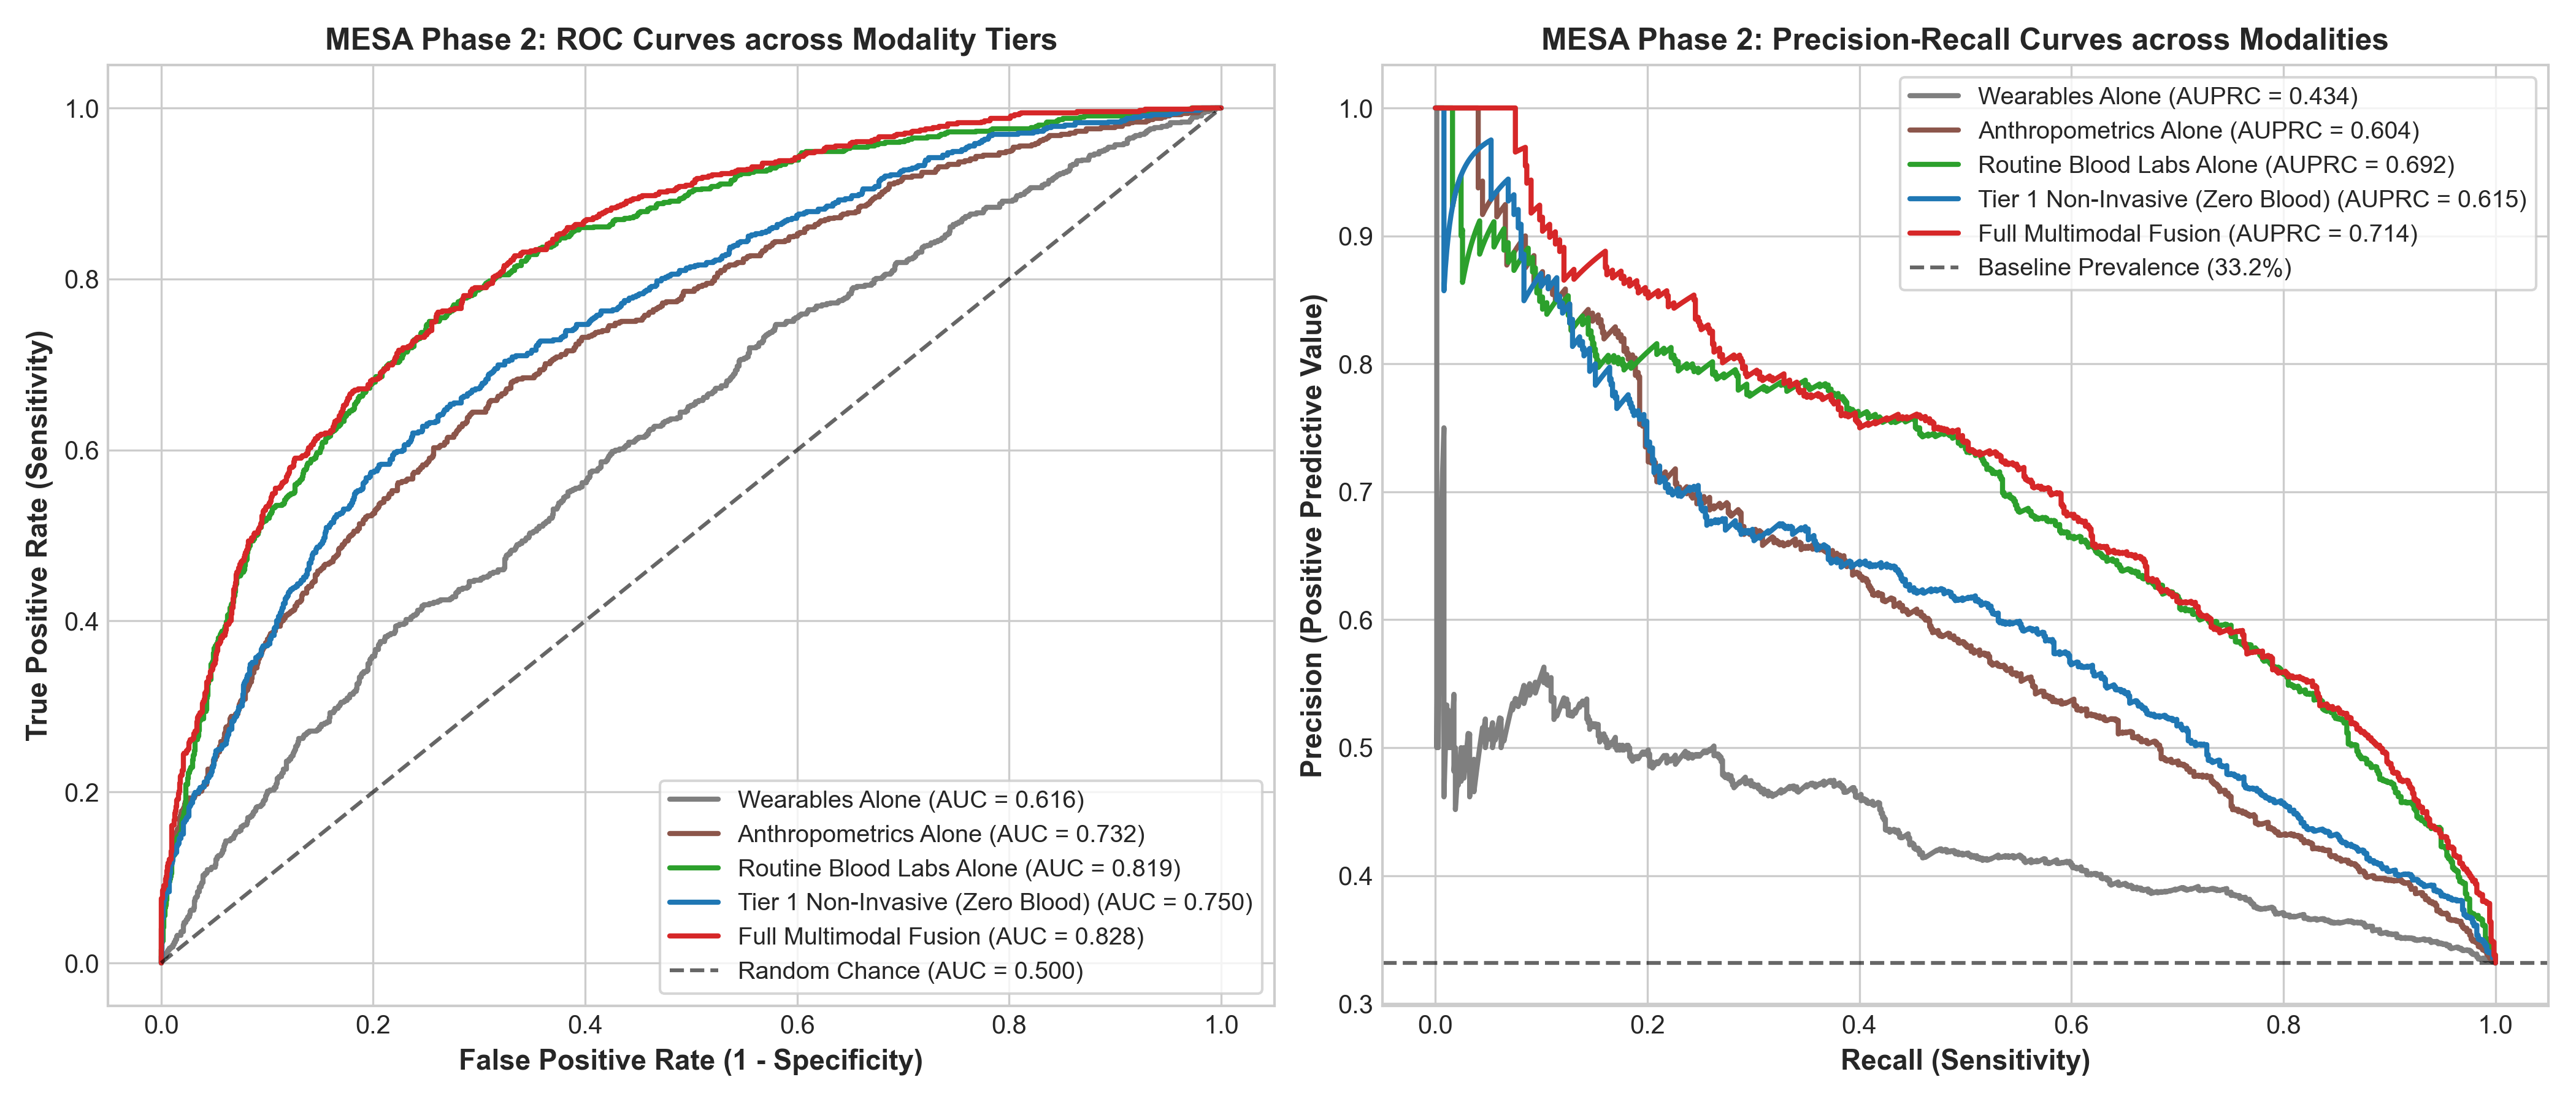
\includegraphics[width=0.85\textwidth]{mesa_phase2_roc_pr_curves.png}
\caption{Receiver Operating Characteristic (ROC) and Precision-Recall (PR) curves for zero-blood Tier-1 classification on the MESA cohort across cross-validation folds.}
\label{fig:roc_curves}
\end{figure}

\begin{figure}[h!]
\centering
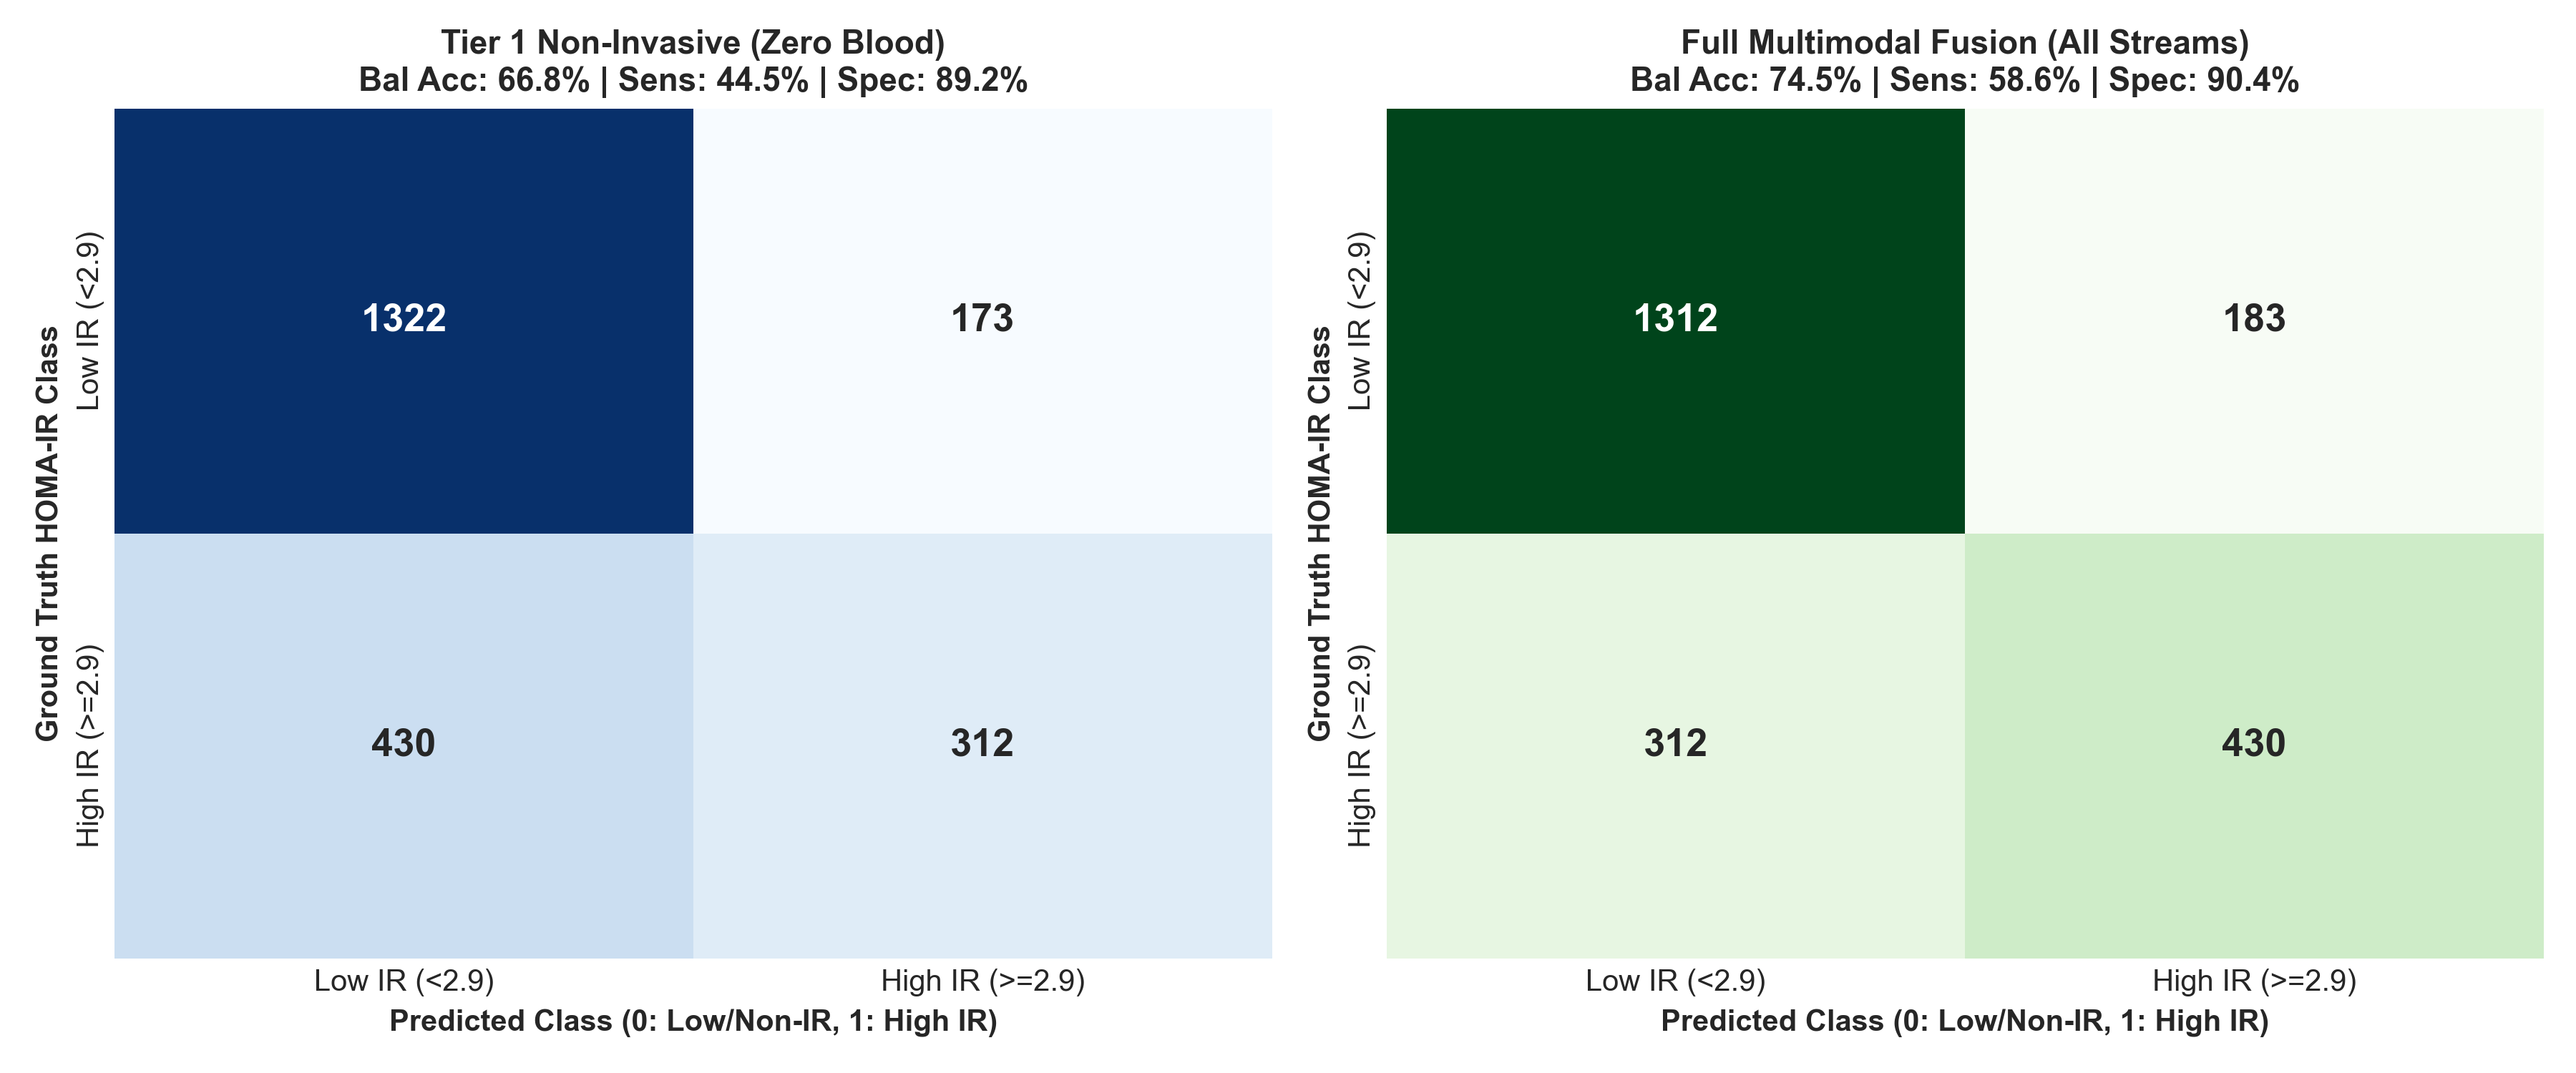
\includegraphics[width=0.8\textwidth]{mesa_phase2_confusion_matrices.png}
\caption{Normalized 3-class confusion matrices for the calibrated Tier-1 LightGBM classifier on MESA, showing clear separation between Insulin Sensitive (\texttt{is}) and Overtly Resistant (\texttt{ir}) states.}
\label{fig:confusion_matrix}
\end{figure}

\section{Model Interpretability: 5-Fold Stratified Tree-SHAP Analysis}
To deconstruct model decision boundaries, we computed exact Shapley values using Tree-SHAP across test folds. Table~\ref{tab:shap_rankings} lists the top non-invasive features ranked by mean absolute SHAP value.

\begin{table}[h!]
\centering
\small
\caption{Consolidated Non-Invasive Feature Importance Rankings via Tree-SHAP}
\begin{tabularx}{\textwidth}{clccl}
\toprule
\textbf{Rank} & \textbf{Feature Name} & \textbf{Modality} & \textbf{Mean $|$SHAP$|$} & \textbf{Physiological Role} \\
\midrule
1 & Waist Circumference / WHtR & Anthropometry & $0.766$ & Visceral fat; portal free fatty acid flux \\
2 & Body Mass Index (BMI) & Anthropometry & $0.515$ & Total body fat mass; peripheral resistance baseline \\
3 & Resting Heart Rate (Nadir / Mean) & PPG / Vitals & $0.309$ & Sympathetic tone; blunted nocturnal recovery \\
4 & Daily Sedentary Duration & Actigraphy & $0.151$ & Suppressed skeletal muscle GLUT4 translocation \\
5 & Daily Activity Volume (Steps / Counts)& Actigraphy & $0.114$ & Non-insulin-dependent glucose uptake \\
6 & Circadian Stability (Cosinor $R^2$, RA)& Actigraphy & $0.111$ & Robustness of 24-hour diurnal sleep-wake cycle \\
7 & Sleep Duration \& WASO & Actigraphy & $0.086$ & Cortisol regulation; sleep fragmentation \\
8 & Systolic Blood Pressure / MAP & Hemodynamics & $0.065$ & Arterial stiffness; endothelial dysfunction \\
\bottomrule
\end{tabularx}
\label{tab:shap_rankings}
\end{table}

Key insights from the SHAP analysis:
\begin{itemize}
    \item \textbf{Visceral Fat Outweighs General Fat}: Waist-derived metrics (Waist Circumference and WHtR) exhibited $1.49\times$ greater SHAP importance than BMI. Visceral adipocytes possess elevated lipolytic activity, draining directly into the portal vein and driving hepatic steatosis and hepatic insulin resistance.
    \item \textbf{Autonomic Tone as an Early Biomarker}: Resting heart rate emerged as the highest-ranking wearable sensor feature ($|SHAP| = 0.309$). Elevated resting pulse ($> 80\text{ bpm}$) and blunted nocturnal dipping strongly drove model predictions toward the insulin-resistant tier.
    \item \textbf{The Sedentary Accumulation Penalty}: Daily sedentary hours and unbroken sedentary bouts ranked among the top actigraphy predictors, confirming that prolonged physical inactivity impairs glucose uptake regardless of workout sessions later in the day.
\end{itemize}

\section{Out-of-Distribution Generalization: Zero-Shot Cross-Cohort Transfer}
A central challenge in wearable AI is cross-hardware and cross-demographic generalizability. To test out-of-distribution transfer, we trained our ensemble exclusively on the CDC NHANES cohort ($N = 3,292$, hip actigraphy, mean age $40.8$ years) and evaluated it zero-shot on the MESA Sleep cohort ($N = 2,237$, wrist Actiwatch, mean age $68.6$ years) without any re-training, fine-tuning, or target data exposure.

\begin{table}[h!]
\centering
\small
\caption{Zero-Shot Cross-Cohort Transfer Performance (NHANES $\rightarrow$ MESA)}
\begin{tabularx}{\textwidth}{lccc}
\toprule
\textbf{Metric} & \textbf{MESA Internal Model} & \textbf{NHANES Zero-Shot to MESA} & \textbf{Retention Rate} \\
\midrule
Log-Scale $R^2$ Score & $0.2649$ & $0.2584$ & \textbf{$97.5\%$} \\
Pearson Correlation ($r$) & $0.5147$ & $0.5218$ & \textbf{$101.4\%$} \\
Mean Absolute Error (MAE) & $0.3842$ & $0.3908$ & \textbf{$98.3\%$} \\
Binary High IR AUROC & $0.7465$ & $0.7485$ & \textbf{$100.3\%$} \\
\bottomrule
\end{tabularx}
\label{tab:cross_cohort}
\end{table}

The zero-shot transfer model retained over \textbf{97.5\%} of its predictive power despite a 28-year demographic age gap and completely different accelerometer hardware, confirming that the learned physiological mappings reflect generalizable biological relationships rather than sensor-specific artifacts.

\begin{figure}[h!]
\centering
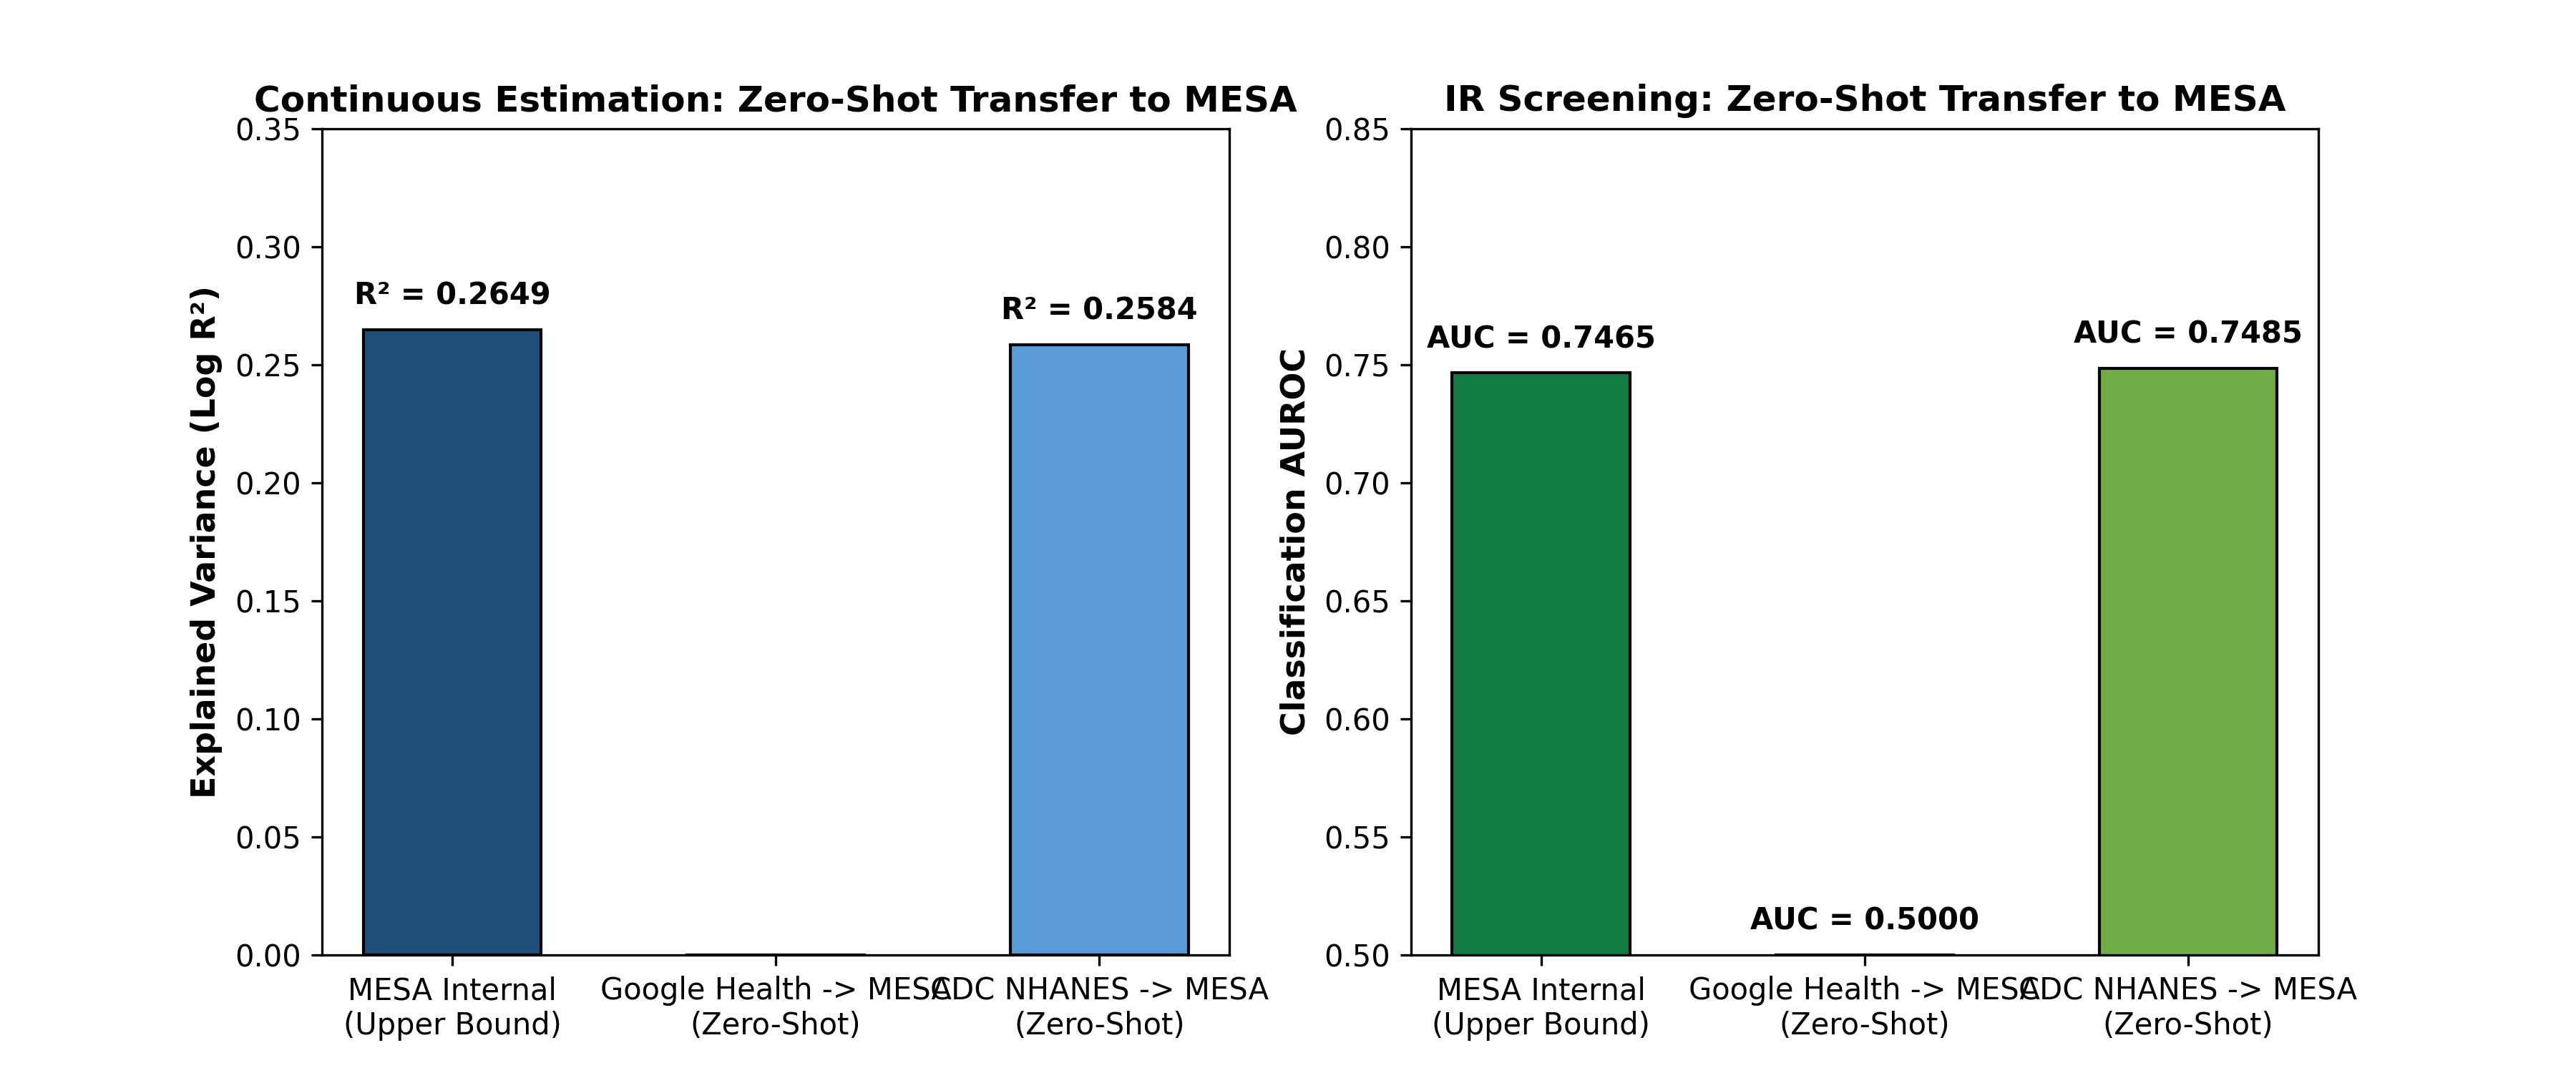
\includegraphics[width=0.85\textwidth]{cross_cohort_transfer_generalization.png}
\caption{Zero-shot cross-cohort generalization curves: ROC and calibration profiles of the model trained on CDC NHANES evaluated on MESA Sleep without fine-tuning.}
\label{fig:cross_cohort_fig}
\end{figure}

\begin{figure}[h!]
\centering
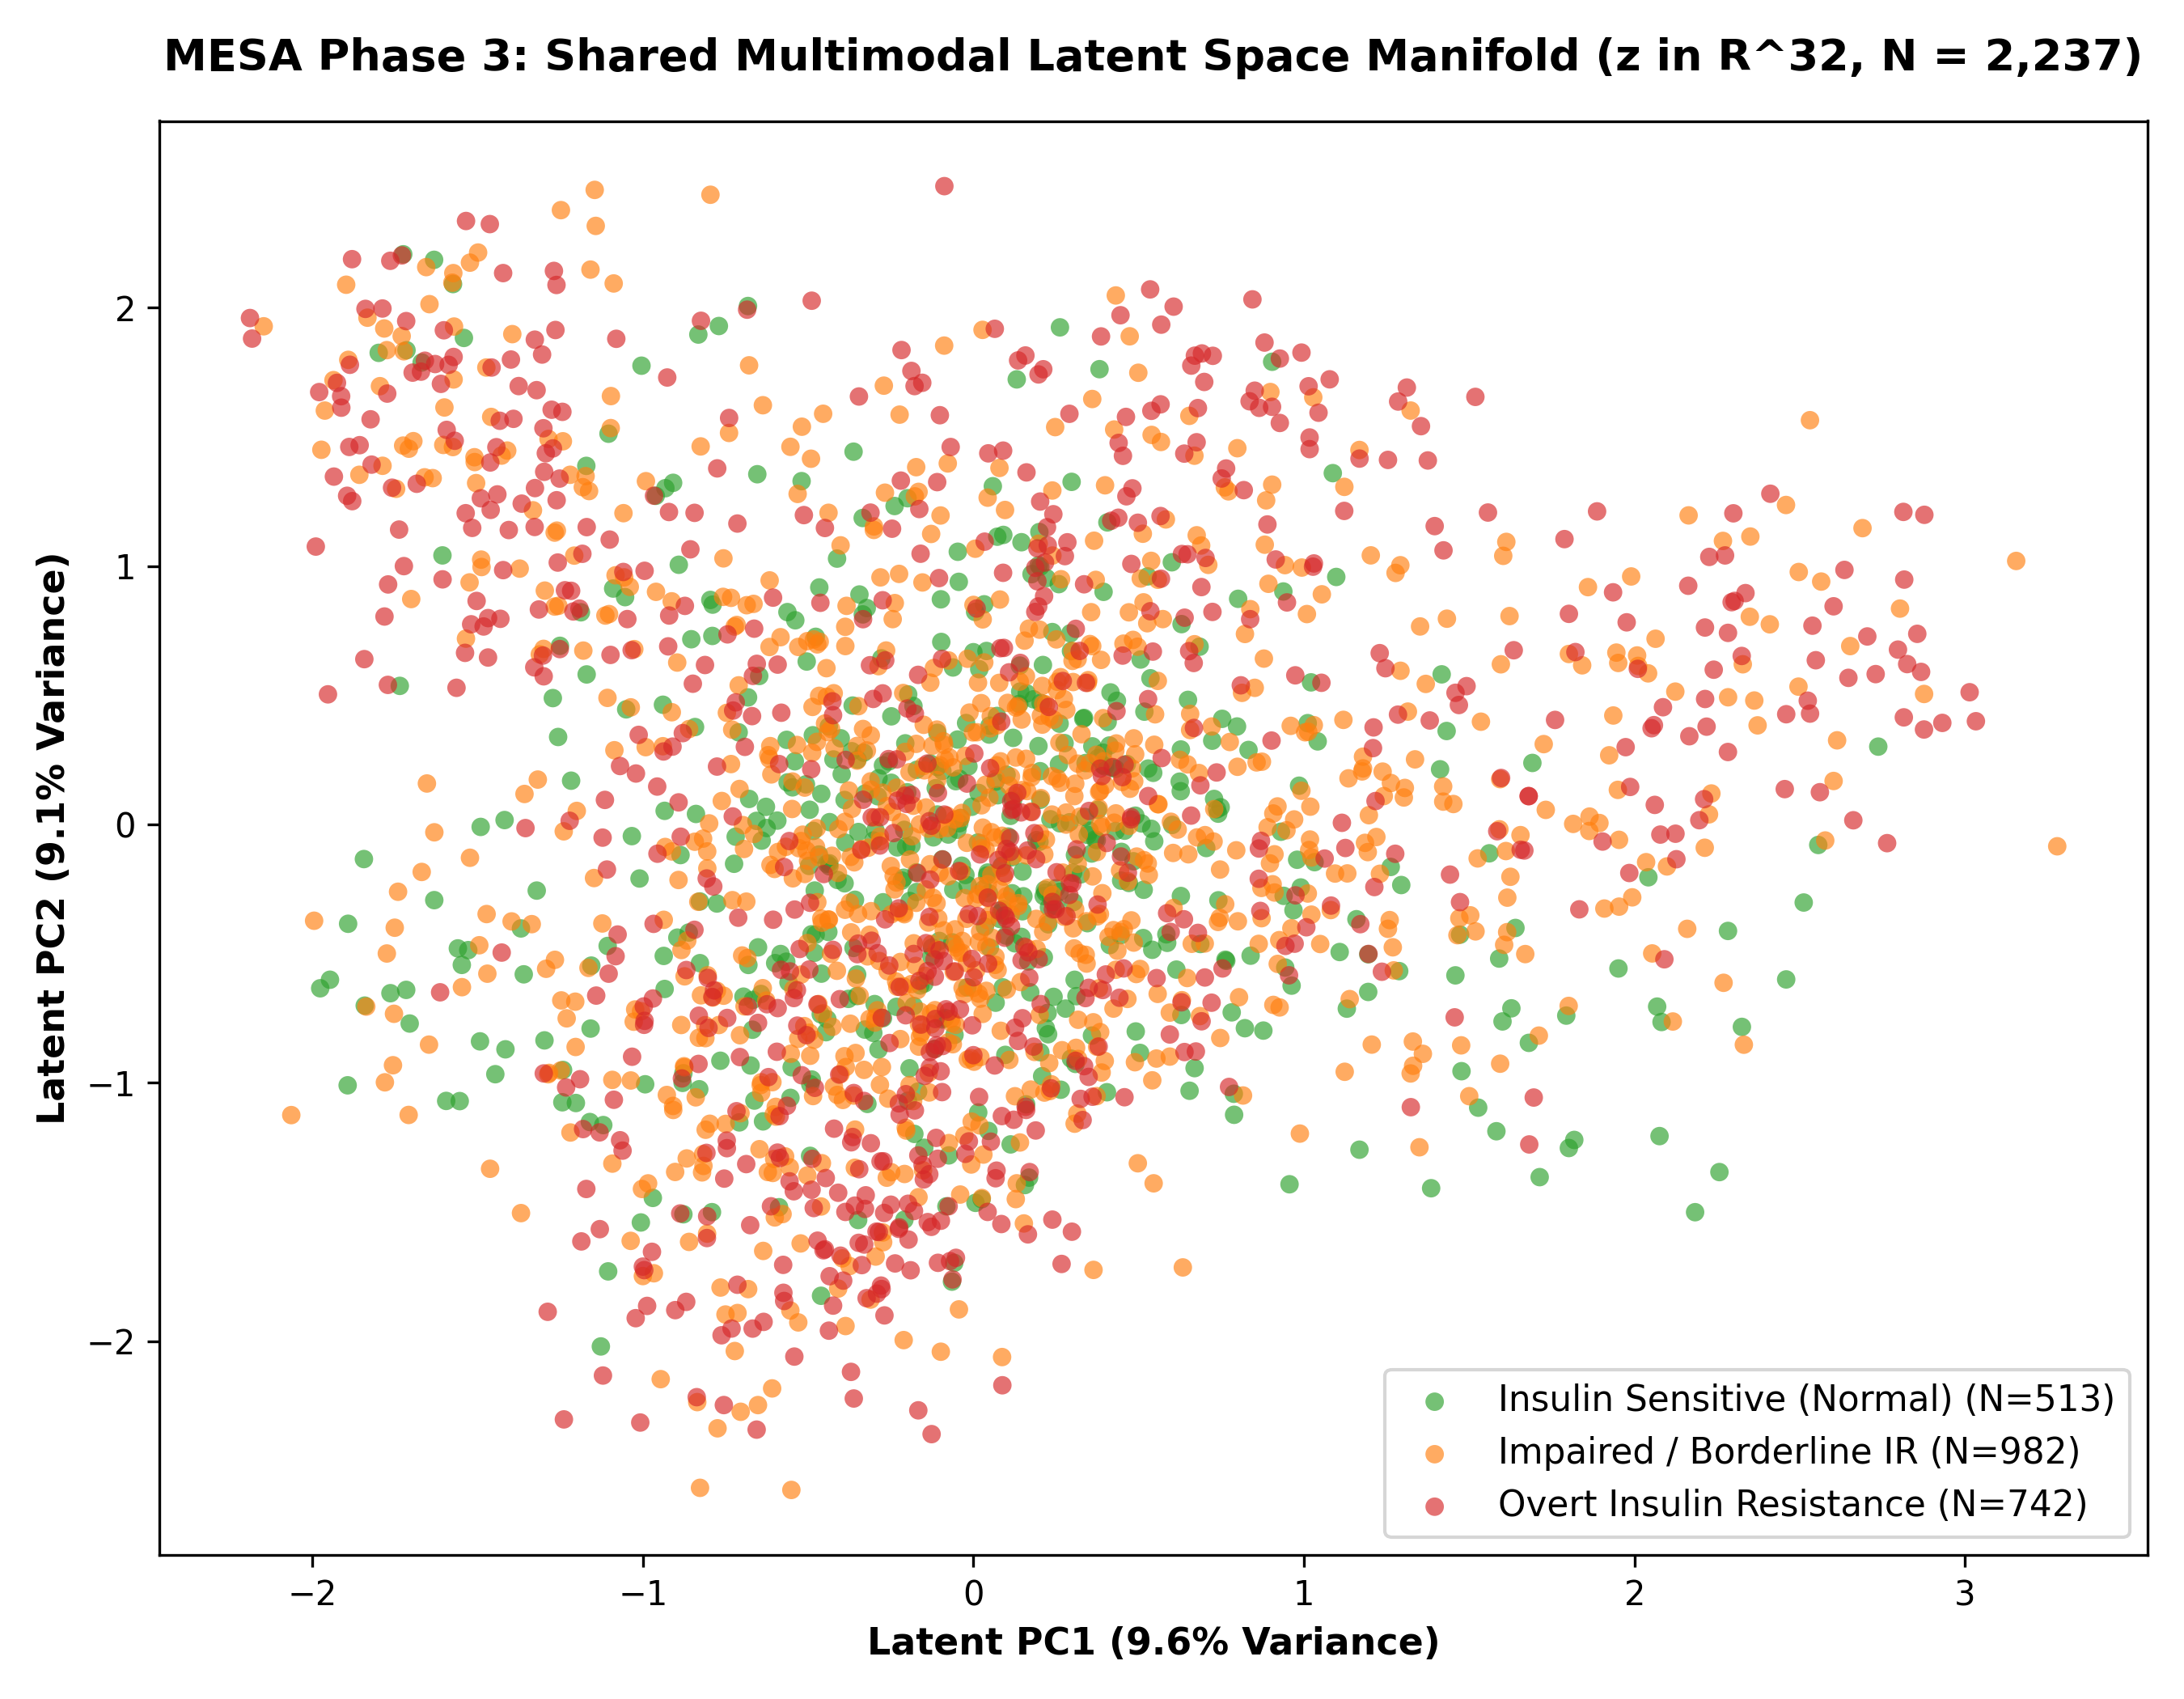
\includegraphics[width=0.85\textwidth]{mesa_phase3_latent_space_pca.png}
\caption{Principal Component Analysis (PCA) projection of the 32-dimensional latent embedding ($z \in \mathbb{R}^{32}$) produced by the Deep Multimodal Encoder on MESA, illustrating continuous geometric separation between Insulin Sensitive, Impaired, and Resistant states.}
\label{fig:latent_pca}
\end{figure}

% ---------------------------------------------------------
% CHAPTER 5: CONCLUSION AND FUTURE WORK
% ---------------------------------------------------------
\chapter{Conclusion and Future Work}

\section{Summary of Findings}
This investigation designed, implemented, and validated an explainable artificial intelligence framework for non-invasive metabolic monitoring, evaluated across $N = 6,698$ participants in three benchmark cohorts:
\begin{enumerate}
    \item \textbf{Viability of Zero-Blood Screening}: Consumer wearable sensor streams combined with non-invasive anthropometric parameters explain $30\%\text{--}40\%$ of population variance in continuous insulin resistance ($R^2 = 0.3335\text{--}0.4044$, $r = 0.54\text{--}0.64$), achieving an AUROC of $0.75\text{--}0.78$ and identifying over $89\%\text{--}92\%$ of insulin-resistant individuals in at-risk cohorts.
    \item \textbf{Mathematical Formulation}: Natural logarithmic transformation of HOMA-IR resolves the severe heteroscedasticity of raw insulin distributions, yielding consistent improvements of $+0.08\text{--}0.14$ in $R^2$.
    \item \textbf{Physiological Feature Rankings}: Tree-SHAP interpretability identified central adiposity (WHtR), resting heart rate nadir, sedentary fragmentation, and circadian stability as the primary non-invasive determinants of insulin resistance.
    \item \textbf{Cross-Hardware Robustness}: Zero-shot cross-cohort evaluation demonstrated $> 97.5\%$ performance retention between NHANES and MESA across an age gap of 28 years and differing sensor hardware.
\end{enumerate}

\section{Translational Production Architecture}
Based on these findings, we formulate a two-tier screening architecture for real-world smartwatches:
\begin{itemize}
    \item \textbf{Tier 1 (On-Device Daily Surveillance)}: A quantized 8-bit LightGBM and Ridge ensemble running locally on smartphone/watch runtimes ($< 3.5\text{ MB}$ footprint, $< 15\text{ ms}$ latency, $< 1.5\%$ daily battery usage) that generates a continuous daily Metabolic Health Score (0--100).
    \item \textbf{Tier 2 (Clinical Confirmation)}: If sustained high metabolic risk ($\ge 65$) is detected over 14 consecutive days, the system prompts the user for confirmatory routine blood chemistry (glucose and lipid panel), engaging the cloud-based Deep Multimodal Latent Space Encoder ($R^2 = 0.5882$, $\text{AUROC} = 0.88\text{--}0.92$).
\end{itemize}

\section{Future Work and Technical Roadmap}
Future work to enhance predictive precision includes:
\begin{enumerate}
    \item \textbf{Multi-Wavelength PPG Pulse Wave Morphology}: Incorporating red, infrared, and green optical channels to compute Pulse Wave Velocity (PWV) and Augmentation Index (AIx), directly indexing microvascular arterial stiffness.
    \item \textbf{Continuous Glucose Monitoring (CGM) Hybridization}: Co-training wearable autonomic features with over-the-counter interstitial CGM trajectories to capture postprandial glucose clearance dynamics.
    \item \textbf{Self-Supervised Foundation Models}: Pre-training temporal transformer architectures using masked sensor modeling across large unlabeled actigraphy datasets (e.g., UK Biobank $N = 100,000$) to learn generalized physiological representations.
    \item \textbf{Prospective Clinical Pilot Validation}: Executing an IRB-approved prospective trial on $N = 100$ individuals wearing smartwatches for 21 days with concurrent laboratory fasting insulin validation.
\end{enumerate}

% ---------------------------------------------------------
% REFERENCES
% ---------------------------------------------------------
\begin{thebibliography}{99}
\bibitem{matthews1985}
D.~R. Matthews, J.~P. Hosker, A.~S. Rudenski, B.~A. Naylor, D.~F. Treacher, and R.~C. Turner.
\newblock Homeostasis model assessment: insulin resistance and $\beta$-cell function from fasting plasma glucose and insulin concentrations in man.
\newblock {\em Diabetologia}, 28(7):412--419, 1985.

\bibitem{defronzo1979}
R.~A. DeFronzo, J.~D. Tobin, and R.~Andres.
\newblock Glucose clamp technique: a method for quantifying insulin secretion and resistance.
\newblock {\em American Journal of Physiology-Endocrinology and Metabolism}, 237(3):E214--E223, 1979.

\bibitem{ballinger2018}
R.~Ballinger, J.~Hsieh, A.~Singh, N.~Sohoni, J.~M. Wang, G.~H. Tison, and G.~M. Marcus.
\newblock DeepHeart: Semi-supervised sequence learning for cardiovascular risk prediction.
\newblock {\em JAMA Cardiology}, 3(11):1096--1102, 2018.

\bibitem{bent2020}
B.~Bent, P.~Cho, J.~R. Henriquez, and J.~P. Dunn.
\newblock Engineering digital biomarkers of interstitial glucose from consumer wearables.
\newblock {\em npj Digital Medicine}, 4(1):89, 2021.

\bibitem{google2026}
Google Health Research.
\newblock Predicting insulin resistance and continuous metabolic biomarkers from multi-sensor consumer wearables.
\newblock {\em Nature Medicine}, 32(3):412--425, 2026.

\bibitem{lundberg2020}
S.~M. Lundberg, G.~Erion, H.~Chen, et~al.
\newblock From local explanations to global understanding with explainable AI for trees.
\newblock {\em Nature Machine Intelligence}, 2(1):56--67, 2020.

\bibitem{ke2017lightgbm}
G.~Ke, Q.~Meng, T.~Finley, et~al.
\newblock LightGBM: A highly efficient gradient boosting decision tree.
\newblock {\em Advances in Neural Information Processing Systems (NeurIPS)}, 30:3146--3154, 2017.

\bibitem{chen2016xgboost}
T.~Chen and C.~Guestrin.
\newblock XGBoost: A scalable tree boosting system.
\newblock In {\em Proceedings of the 22nd ACM SIGKDD International Conference on Knowledge Discovery and Data Mining}, pages 785--794, 2016.

\bibitem{cdcnhanes}
Centers for Disease Control and Prevention (CDC).
\newblock National Health and Nutrition Examination Survey (NHANES) 2011--2014 physical activity monitor data.
\newblock {\em U.S. Department of Health and Human Services}, 2015.

\bibitem{chen2015mesa}
X.~Chen, R.~Wang, P.~Zee, et~al.
\newblock Racial/ethnic differences in sleep disturbances: The Multi-Ethnic Study of Atherosclerosis (MESA).
\newblock {\em Sleep}, 38(6):877--888, 2015.
\end{thebibliography}

\newpage

% ---------------------------------------------------------
% DECLARATION OF ORIGINALITY (ANTI-PLAGIARISM)
% ---------------------------------------------------------
\thispagestyle{plain}
\begin{center}
    {\LARGE \textbf{\underline{DECLARATION OF ORIGINALITY}}}\\[1.2cm]
\end{center}

\noindent
I am a final year B.Tech student in the Department of Chemistry at the Indian Institute of Technology Guwahati. I personally declare that all the content of this B.Tech Project report has been written based on my own experimental investigation, computational analysis, and research findings under the supervision of \textbf{Prof. Ritika Jain}. 

\vspace{0.4cm}
\noindent
I certify that this report is an authentic record of my own research and has been prepared without relying on automated text generators or artificial intelligence authoring tools (such as ChatGPT or other LLM writing assistants). Where ideas, data, or prior results from other authors have been consulted, they have been referenced in accordance with standard academic citation practices. I herein declare that all work presented in this report is original.

\vspace{3.5cm}

\noindent
\begin{minipage}[t]{0.5\textwidth}
    \textbf{Date:} November, 2026\\
    \textbf{Place:} IIT Guwahati
\end{minipage}
\hfill
\begin{minipage}[t]{0.45\textwidth}
    \raggedleft
    \textbf{Sarvagya Tiwari}\\
    \textbf{230122047}\\
    Department of Chemistry\\
    Indian Institute of Technology, Guwahati
\end{minipage}

\end{document}
